\section{Report}\label{report}

\begin{quote}
Trang bìa
\end{quote}

\begin{itemize}
\itemsep1pt\parskip0pt\parsep0pt
\item
  Tên học phần: Kĩ thuật lập trình
\item
  Giảng viên hướng dẫn: Nguyễn Thị Thanh Huyền
\item
  Nhóm sinh viên thực hiện: Nhóm 2 lớp

  \begin{itemize}
  \itemsep1pt\parskip0pt\parsep0pt
  \item
    An Việt Trung 20195936
  \item
    Lê Thị Kiều Trang 20195930
  \end{itemize}
\item
  Logo Trường + Viện
\end{itemize}

\section{Mục lục}\label{mux1ee5c-lux1ee5c}

\section{I. Quá trình phát triển Chương
trình}\label{i.-quuxe1-truxecnh-phuxe1t-triux1ec3n-chux1b0ux1a1ng-truxecnh}

\subsection{Bước 0: Phân tích thiết kế chương
trình}\label{bux1b0ux1edbc-0-phuxe2n-tuxedch-thiux1ebft-kux1ebf-chux1b0ux1a1ng-truxecnh}

\subsubsection{Thiết kế chức năng tìm
nghiệm}\label{thiux1ebft-kux1ebf-chux1ee9c-nux103ng-tuxecm-nghiux1ec7m}

\begin{figure}[htbp]
\centering
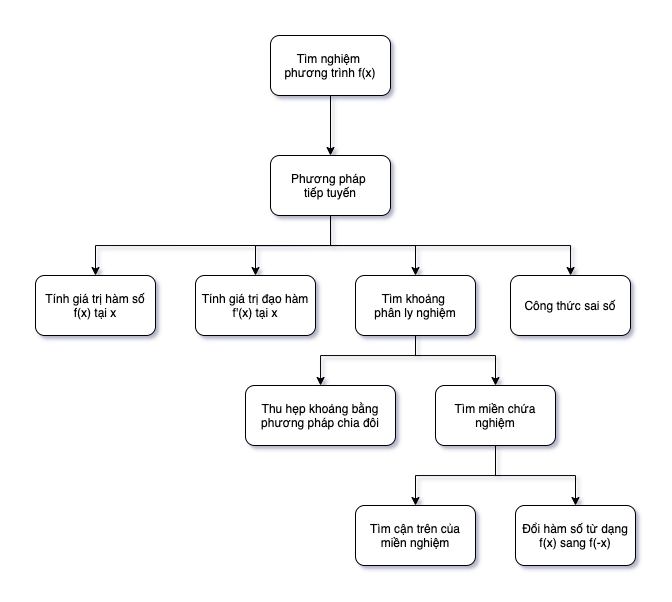
\includegraphics{Report 217e2873af07496eaa16f4f8701bd590/find_root.png}
\caption{Report\%20217e2873af07496eaa16f4f8701bd590/find\_root.png}
\end{figure}

\subsubsection{Thiết kế chức năng
in}\label{thiux1ebft-kux1ebf-chux1ee9c-nux103ng-in}

\begin{itemize}
\item
  Gửi nội dung xâu

  → In ra màn hình xâu

  → In ra file xâu
\end{itemize}

\subsection{Bước 1: Mô tả chương trình
chính}\label{bux1b0ux1edbc-1-muxf4-tux1ea3-chux1b0ux1a1ng-truxecnh-chuxednh}

\subsubsection{Các cấu trúc dữ
liệu}\label{cuxe1c-cux1ea5u-truxfac-dux1eef-liux1ec7u}

\begin{Shaded}
\begin{Highlighting}[]
\CommentTok{// Kiểu miền}
\KeywordTok{typedef} \KeywordTok{struct} \NormalTok{Interval \{}
    \DataTypeTok{double} \NormalTok{left;  }\CommentTok{// Giới hạn trái}
    \DataTypeTok{double} \NormalTok{right; }\CommentTok{// Giới hạn phải}
\NormalTok{\} Interval;}

\CommentTok{// Hạng tử trong đa thức}
\KeywordTok{typedef} \KeywordTok{struct} \NormalTok{PNode \{}
    \DataTypeTok{double} \NormalTok{coeff; }\CommentTok{// Hệ số}
    \DataTypeTok{int} \NormalTok{exponent; }\CommentTok{// Bậc}

    \NormalTok{PNode* next;  }\CommentTok{// Hạng tử tiếp theo}
\NormalTok{\} PNode;}

\CommentTok{// Đa thức}
\KeywordTok{class} \NormalTok{Polynomial \{}
\KeywordTok{private}\NormalTok{:}
    \NormalTok{PNode* head;            }\CommentTok{// Danh sách các hạng tự}
    \NormalTok{Interval root_interval; }\CommentTok{// Miền chứa nghiệm}

    \DataTypeTok{bool} \NormalTok{found_root_interval; }\CommentTok{// đánh dấu để không tìm lại miền nghiệm nhiều lần}
\NormalTok{\}}
\end{Highlighting}
\end{Shaded}

\subsubsection{Hàm main}\label{huxe0m-main}

\begin{itemize}
\itemsep1pt\parskip0pt\parsep0pt
\item
  Thực thi hàm đọc file \textbf{``project-settings.txt''} và khởi tạo
  các giá trị global cho chương trình, gồm có:

  \begin{itemize}
  \itemsep1pt\parskip0pt\parsep0pt
  \item
    Đường dẫn đến \textbf{file input:} chứa thông tin về đa thức
  \item
    Đường dẫn đến \textbf{file output:} chứa ****quá trình thực hiện
    chương trình và các kết quả ra
  \item
    Các hằng số mặc định

    \begin{itemize}
    \itemsep1pt\parskip0pt\parsep0pt
    \item
      Số chữ số thập phân sau dấu phẩy
    \item
      Hằng số Epsilon
    \end{itemize}
  \end{itemize}
\item
  Khởi tạo đa thức f(x) từ file input
\item
  Thực thi thân chương trình chính (vòng lặp):

  \begin{itemize}
  \itemsep1pt\parskip0pt\parsep0pt
  \item
    In lên màn hình các lựa chọn chức năng hiện tại của chương trình
    (chi tiết các chức năng phía dưới)
  \item
    Đợi người dùng chọn chức năng muốn sử dụng
  \item
    In ra tên chức năng người dùng lựa chọn
  \item
    Thực thi chức năng người dùng lựa chọn
  \end{itemize}
\item
  Thực thi hàm kết thúc chương trình (đóng file, giải phóng vùng
  nhớ,\ldots{})
\end{itemize}

\subsubsection{Các chức năng trong
menu}\label{cuxe1c-chux1ee9c-nux103ng-trong-menu}

\begin{enumerate}
\def\labelenumi{\arabic{enumi}.}
\itemsep1pt\parskip0pt\parsep0pt
\item
  Tìm miền chứa nghiệm

  \begin{itemize}
  \itemsep1pt\parskip0pt\parsep0pt
  \item
    Sử dụng hàm \textbf{Get\_Root\_Interval}
  \item
    In kết quả
  \end{itemize}
\item
  Tìm các khoảng phân ly $(a,b)$ thoả mãn $|b-a| \leq 0,5$

  \begin{itemize}
  \itemsep1pt\parskip0pt\parsep0pt
  \item
    Sử dùng hàm \textbf{Find\_KPL} với giá trị $0,5$
  \item
    In kết quả
  \end{itemize}
\item
  Tìm nghiệm gần đúng với số lần lặp $n$

  \begin{itemize}
  \itemsep1pt\parskip0pt\parsep0pt
  \item
    Nhập $n$
  \item
    Nhập khoảng và kiểm tra xem có phân ly
  \item
    Sử dụng hàm \textbf{Newton\_Raphson} với số lần lặp $n$
  \item
    In kết quả
  \end{itemize}
\item
  Tìm nghiệm gần đúng với sai số $\epsilon$

  \begin{itemize}
  \itemsep1pt\parskip0pt\parsep0pt
  \item
    Nhập $\epsilon$
  \item
    Nhập khoảng và kiểm tra xem có phân ly
  \item
    Sử dụng hàm \textbf{Newton\_Raphson\_Err\_Formula} với sai số
    $\epsilon$
  \item
    In kết quả
  \end{itemize}
\item
  Tìm nghiệm gần đúng $x_n$ thoả mãn $|x_n -x_{n-1}|\leq \epsilon$

  \begin{itemize}
  \itemsep1pt\parskip0pt\parsep0pt
  \item
    Nhập $\epsilon$
  \item
    Nhập khoảng và kiểm tra xem có phân ly
  \item
    Sử dụng hàm \textbf{Newton\_Raphson} với sai số $\epsilon$
  \item
    In kết quả
  \end{itemize}
\end{enumerate}

\subsection{Bước 2: Chi tiết các Module
chính}\label{bux1b0ux1edbc-2-chi-tiux1ebft-cuxe1c-module-chuxednh}

\subsubsection{Tìm cận trên của miền
nghiệm}\label{tuxecm-cux1eadn-truxean-cux1ee7a-miux1ec1n-nghiux1ec7m}

\begin{Shaded}
\begin{Highlighting}[]
\DataTypeTok{double} \NormalTok{Polynomial::Find_Root_Interval_Upper_Edge() \{}
    \KeywordTok{if} \NormalTok{(head == NULL) }\KeywordTok{return} \DecValTok{0}\NormalTok{;}

    \CommentTok{// sign of a0}
    \DataTypeTok{double} \NormalTok{sign = head->coeff < }\DecValTok{0} \NormalTok{? -}\FloatTok{1.}\NormalTok{0f : }\FloatTok{1.}\NormalTok{0f;}
    \DataTypeTok{int} \NormalTok{m = -}\DecValTok{1}\NormalTok{;}
    \DataTypeTok{double} \NormalTok{max;}
    \NormalTok{PNode* cur = head->next;}

    \KeywordTok{while} \NormalTok{(cur != NULL) \{}
        \KeywordTok{if} \NormalTok{(cur->coeff * sign < }\DecValTok{0}\NormalTok{) \{}
            \NormalTok{m = head->exponent - cur->exponent;}
            \NormalTok{max = cur->coeff;}
            \KeywordTok{break}\NormalTok{;}
        \NormalTok{\}}
        \NormalTok{cur = cur->next;}
    \NormalTok{\}}

    \CommentTok{// opposite sign coeffect is available}
    \KeywordTok{if} \NormalTok{(m >= }\DecValTok{0}\NormalTok{) \{}
        \NormalTok{cur = head->next;}
        \KeywordTok{while} \NormalTok{(cur != NULL) \{}
            \KeywordTok{if} \NormalTok{(cur->coeff * sign < }\DecValTok{0}\NormalTok{) \{}
                \KeywordTok{if} \NormalTok{(fabs(cur->coeff) > fabs(max))}
                    \NormalTok{max = cur->coeff;}
            \NormalTok{\}}

            \NormalTok{cur = cur->next;}
        \NormalTok{\}}
        
        \KeywordTok{return} \DecValTok{1} \NormalTok{+ pow(-max / head->coeff, }\FloatTok{1.}\NormalTok{0f / m);}
    \NormalTok{\} }\KeywordTok{else} \NormalTok{\{}
        \KeywordTok{return} \DecValTok{0}\NormalTok{;}
    \NormalTok{\}}
\NormalTok{\}}
\end{Highlighting}
\end{Shaded}

\subsubsection{Đổi hàm số từ dạng f(x) sang
f(-x)}\label{ux111ux1ed5i-huxe0m-sux1ed1-tux1eeb-dux1ea1ng-fx-sang-f-x}

\begin{Shaded}
\begin{Highlighting}[]
\DataTypeTok{void} \NormalTok{Polynomial::Reverse_Odd_Exponent_Sign() \{}
    \NormalTok{PNode* cur = head;}
    \KeywordTok{while} \NormalTok{(cur != NULL) \{}
        \KeywordTok{if} \NormalTok{(cur->exponent % }\DecValTok{2} \NormalTok{== }\DecValTok{1}\NormalTok{)}
            \NormalTok{cur->coeff = -cur->coeff;}
        \NormalTok{cur = cur->next;}
    \NormalTok{\}}
\NormalTok{\}}
\end{Highlighting}
\end{Shaded}

\subsubsection{Tìm miền chứa
nghiệm}\label{tuxecm-miux1ec1n-chux1ee9a-nghiux1ec7m}

\begin{Shaded}
\begin{Highlighting}[]
\DataTypeTok{void} \NormalTok{Polynomial::Find_Root_Interval() \{}
    \NormalTok{root_interval.right = Find_Root_Interval_Upper_Edge();}

    \CommentTok{// Temporary change f(x) to f(-x)}
    \NormalTok{Reverse_Odd_Exponent_Sign();}

    \NormalTok{root_interval.left = -Find_Root_Interval_Upper_Edge();}

    \CommentTok{// Change back to f(x)}
    \NormalTok{Reverse_Odd_Exponent_Sign();}

    \NormalTok{found_root_interval = }\KeywordTok{true}\NormalTok{;}
\NormalTok{\}}
\end{Highlighting}
\end{Shaded}

\subsubsection{Thu hẹp khoảng bằng phương pháp chia
đôi}\label{thu-hux1eb9p-khoux1ea3ng-bux1eb1ng-phux1b0ux1a1ng-phuxe1p-chia-ux111uxf4i}

\begin{Shaded}
\begin{Highlighting}[]
\NormalTok{Interval Bisection(Polynomial* f, }\DataTypeTok{double} \NormalTok{a, }\DataTypeTok{double} \NormalTok{b, }\DataTypeTok{double} \NormalTok{dist) \{}
    \NormalTok{Interval res;}
    \DataTypeTok{double} \NormalTok{c = }\DecValTok{0}\NormalTok{;}
    \KeywordTok{while} \NormalTok{(fabs(a - b) > dist) \{}
        \NormalTok{c = (a + b) / }\DecValTok{2}\NormalTok{;}
        \KeywordTok{if} \NormalTok{( sign(f->F(c)) == sign(f->F(b)) )}
            \NormalTok{b = c;}
        \KeywordTok{else}
            \NormalTok{a = c;}
    \NormalTok{\}}

    \NormalTok{res.left = a;}
    \NormalTok{res.right = b;}

    \KeywordTok{return} \NormalTok{res;}
\NormalTok{\}}
\end{Highlighting}
\end{Shaded}

\subsubsection{Tìm khoảng phân ly
nghiệm}\label{tuxecm-khoux1ea3ng-phuxe2n-ly-nghiux1ec7m}

\begin{Shaded}
\begin{Highlighting}[]
\DataTypeTok{void} \NormalTok{Polynomial::Find_KPL(}\DataTypeTok{double} \NormalTok{e) \{}
    \NormalTok{Interval ri = Get_Root_Interval();}
    \DataTypeTok{double} \NormalTok{k = (ri.right - ri.left) / head->exponent;}
    \DataTypeTok{double} \NormalTok{A = ri.left;}
    \DataTypeTok{double} \NormalTok{B = ri.right;}

    \NormalTok{Interval sInter;}
    \DataTypeTok{int} \NormalTok{count = }\DecValTok{0}\NormalTok{;}

    \KeywordTok{while} \NormalTok{(A <= B) \{}
        \KeywordTok{if} \NormalTok{(F(A) * F(A + k) < }\DecValTok{0}\NormalTok{) \{}
            \NormalTok{print(}\StringTok{"}\CharTok{\textbackslash{}t}\StringTok{KPL %d ban đầu là (%lf, %lf)}\CharTok{\textbackslash{}n}\StringTok{"}\NormalTok{, ++count, A, A + k);}
            \NormalTok{sInter.left = A;}
            \NormalTok{sInter.right = A + k;}
            \NormalTok{Bisection(}\KeywordTok{this}\NormalTok{, &sInter, e);}
            \NormalTok{print(}\StringTok{"}\CharTok{\textbackslash{}t}\StringTok{KPL %d sau khi thu hẹp bằng PP chia đôi là (%lf, %lf)}\CharTok{\textbackslash{}n\textbackslash{}n}\StringTok{"}\NormalTok{, count, sInter.left, sInter.right);}
        \NormalTok{\}}
        \NormalTok{A = A + k;}
    \NormalTok{\}}
\NormalTok{\}}
\end{Highlighting}
\end{Shaded}

\subsubsection{Công thức sai số}\label{cuxf4ng-thux1ee9c-sai-sux1ed1}

\begin{Shaded}
\begin{Highlighting}[]
\DataTypeTok{double} \NormalTok{Polynomial::Err_Target_Form(}\DataTypeTok{double} \NormalTok{x, }\DataTypeTok{double} \NormalTok{m) \{}
    \KeywordTok{return} \NormalTok{fabs(F(x) / m);}
\NormalTok{\}}

\DataTypeTok{double} \NormalTok{Polynomial::Err_DA_Form(}\DataTypeTok{double} \NormalTok{x, }\DataTypeTok{double} \NormalTok{px, }\DataTypeTok{double} \NormalTok{m, }\DataTypeTok{double} \NormalTok{M) \{}
    \KeywordTok{return} \NormalTok{(M - m) * fabs(x - px) / m;}
\NormalTok{\}}
\end{Highlighting}
\end{Shaded}

\subsubsection{Tính giá trị hàm số f(x) và đạo hàm f'(x) tại
x}\label{tuxednh-giuxe1-trux1ecb-huxe0m-sux1ed1-fx-vuxe0-ux111ux1ea1o-huxe0m-fx-tux1ea1i-x}

\begin{Shaded}
\begin{Highlighting}[]
\DataTypeTok{double} \NormalTok{Polynomial::F(}\DataTypeTok{double} \NormalTok{x) \{}
    \KeywordTok{if} \NormalTok{(head == NULL) }\KeywordTok{return} \DecValTok{0}\NormalTok{;}

    \DataTypeTok{double} \NormalTok{res = head->coeff;}
    \DataTypeTok{int} \NormalTok{degree = head->exponent;}
    \NormalTok{PNode* cur = head->next;}

    \KeywordTok{while} \NormalTok{(cur != NULL) \{}
        \KeywordTok{while} \NormalTok{(cur->exponent < degree}\DecValTok{-1}\NormalTok{) \{}
            \NormalTok{res *= x;}
            \NormalTok{degree--;}
        \NormalTok{\}}
        \NormalTok{res = cur->coeff + res * x;}
        \NormalTok{degree--;}

        \NormalTok{cur = cur->next;}
    \NormalTok{\}}

    \KeywordTok{return} \NormalTok{res;}
\NormalTok{\}}

\DataTypeTok{double} \NormalTok{Polynomial::dF(}\DataTypeTok{double} \NormalTok{x) \{}
    \KeywordTok{if} \NormalTok{(head == NULL) }\KeywordTok{return} \DecValTok{0}\NormalTok{;}

    \DataTypeTok{double} \NormalTok{res = head->coeff * head->exponent;}
    \DataTypeTok{int} \NormalTok{degree = head->exponent}\DecValTok{-1}\NormalTok{;}
    \NormalTok{PNode* cur = head->next;}

    \KeywordTok{while} \NormalTok{(cur != NULL) \{}
        \KeywordTok{while} \NormalTok{(cur->exponent < degree}\DecValTok{-1}\NormalTok{) \{}
            \NormalTok{res *= x;}
            \NormalTok{degree--;}
        \NormalTok{\}}
        \NormalTok{res = cur->coeff * cur->exponent + res * x;}
        \NormalTok{degree--;}

        \NormalTok{cur = cur->next;}
    \NormalTok{\}}

    \KeywordTok{return} \NormalTok{res;}
\NormalTok{\}}
\end{Highlighting}
\end{Shaded}

\subsubsection{Thuật toán tiếp tuyến
(gốc)}\label{thuux1eadt-touxe1n-tiux1ebfp-tuyux1ebfn-gux1ed1c}

\begin{Shaded}
\begin{Highlighting}[]
\DataTypeTok{double} \NormalTok{Newton_Raphson(Polynomial* f, }\DataTypeTok{double} \NormalTok{a, }\DataTypeTok{double} \NormalTok{b, }\DataTypeTok{double} \NormalTok{e) \{}
    \DataTypeTok{double} \NormalTok{x = a;}
    \DataTypeTok{double} \NormalTok{px = }\DecValTok{0}\NormalTok{;}

    \KeywordTok{do} \NormalTok{\{}
        \NormalTok{px = x;}
        \NormalTok{x = x - f->F(x) / f->dF(x);}

    \NormalTok{\} }\KeywordTok{while} \NormalTok{(fabs(x - px) > e);}

    \KeywordTok{return} \NormalTok{x;}
\NormalTok{\}}
\end{Highlighting}
\end{Shaded}

\section{II. Mã nguồn}\label{ii.-muxe3-nguux1ed3n}

\subsubsection{system.h}\label{system.h}

\begin{Shaded}
\begin{Highlighting}[]
\OtherTok{#ifndef AVT_SYSTEM}
\OtherTok{#define AVT_SYSTEM}

\OtherTok{#include <iostream>}
\OtherTok{#include <fstream>}
\OtherTok{#include <string>}
\OtherTok{#include <math.h>}
\OtherTok{#include <unistd.h>}
\OtherTok{#include <ctime>}
\OtherTok{#include <map>}

\OtherTok{#ifdef _WIN32}
\OtherTok{#include <conio.h>}
\OtherTok{#include <windows.h>}
\OtherTok{#endif}

\KeywordTok{using} \KeywordTok{namespace} \NormalTok{std;}

\KeywordTok{namespace} \NormalTok{avt_sys \{}

\CommentTok{// ============================}
\CommentTok{// SYSTEM CALL}
\CommentTok{// ============================}
    \DataTypeTok{void} \NormalTok{ScrollScreen();}
    \DataTypeTok{void} \NormalTok{CursorToHome();}
    \DataTypeTok{void} \NormalTok{ClearScreen();}
    \DataTypeTok{char} \NormalTok{GetInput();}
    \NormalTok{string avtGetCurrentTime();}

\CommentTok{// ============================}
\CommentTok{// IMPLEMENT}
\CommentTok{// ============================}
    \DataTypeTok{void} \NormalTok{ScrollScreen() }
    \NormalTok{\{ }
        \OtherTok{#ifdef _WIN32}
            \NormalTok{system(}\StringTok{"clear"}\NormalTok{);}
        \OtherTok{#else}
            \NormalTok{cout << }\StringTok{"}\CharTok{\textbackslash{}x1b}\StringTok{[2J"}\NormalTok{; }
        \OtherTok{#endif}
    \NormalTok{\};}
    \DataTypeTok{void} \NormalTok{CursorToHome() }
    \NormalTok{\{}
        \OtherTok{#ifdef _WIN32}
            \NormalTok{COORD p = \{}\DecValTok{0}\NormalTok{, }\DecValTok{0}\NormalTok{\};}
            \NormalTok{SetConsoleCursorPosition( GetStdHandle( STD_OUTPUT_HANDLE ), p);}
        \OtherTok{#else}
            \NormalTok{cout << }\StringTok{"}\CharTok{\textbackslash{}x1b}\StringTok{[H"}\NormalTok{;}
        \OtherTok{#endif }
    \NormalTok{\}}

    \DataTypeTok{void} \NormalTok{ClearScreen()}
    \NormalTok{\{}
        \NormalTok{CursorToHome();}

        \DataTypeTok{int} \NormalTok{lines = }\DecValTok{26}\NormalTok{;}
        \KeywordTok{for}\NormalTok{(}\DataTypeTok{int} \NormalTok{i = }\DecValTok{0}\NormalTok{; i <= lines * }\DecValTok{80}\NormalTok{; i++) \{}
            \NormalTok{putchar(i % }\DecValTok{80} \NormalTok{? ' ' : }\DecValTok{10}\NormalTok{); }\CommentTok{// 10 = [Line Feed]}
        \NormalTok{\}}

        \NormalTok{CursorToHome();}
    \NormalTok{\}}

    \DataTypeTok{char} \NormalTok{GetInput()}
    \NormalTok{\{}
        \OtherTok{#ifdef _WIN32}
            \DataTypeTok{char} \NormalTok{input = getch();}
        \OtherTok{#else}
            \CommentTok{// Set terminal to raw mode }
            \NormalTok{system(}\StringTok{"stty raw"}\NormalTok{); }

            \CommentTok{// Wait for single character }
            \DataTypeTok{char} \NormalTok{input = getchar(); }

            \CommentTok{// Reset terminal to normal "cooked" mode }
            \NormalTok{system(}\StringTok{"stty cooked"}\NormalTok{); }
        \OtherTok{#endif }

      \KeywordTok{return} \NormalTok{input;}
    \NormalTok{\}}

    \DataTypeTok{char}\NormalTok{* GetCurrentTime() }
    \NormalTok{\{}
        \NormalTok{time_t now = time(}\DecValTok{0}\NormalTok{);}
        \KeywordTok{return} \NormalTok{ctime(&now);}
    \NormalTok{\}}
\NormalTok{\}}

\OtherTok{#endif}
\end{Highlighting}
\end{Shaded}

\subsubsection{adv\_print.h}\label{advux5fprint.h}

\begin{Shaded}
\begin{Highlighting}[]
\OtherTok{#ifndef ADV_PRINT}
\OtherTok{#define ADV_PRINT}

\OtherTok{#include <stdio.h>}
\OtherTok{#include <stdarg.h>}
\OtherTok{#include "system.h"}

\OtherTok{#define MAX_N 256}

\KeywordTok{namespace} \NormalTok{adv_print \{}
\CommentTok{// ============================}
\CommentTok{// Khai báo}
\CommentTok{// ============================}
    \CommentTok{// FILE output}
    \DataTypeTok{static} \NormalTok{FILE * fout = NULL;}

    \CommentTok{// Mở file}
    \DataTypeTok{void} \NormalTok{init_output_file(}\DataTypeTok{char} \NormalTok{* fileName, }\DataTypeTok{const} \DataTypeTok{char} \NormalTok{* mode);}
    \CommentTok{// Đóng file}
    \DataTypeTok{void} \NormalTok{close_output_file();}

    \CommentTok{// In ra màn hình và file (nếu có)}
    \DataTypeTok{void} \NormalTok{print(}\DataTypeTok{const} \DataTypeTok{char}\NormalTok{* format, ...);}

    \CommentTok{// In kí tự 'c' n lần ra màn hình và file (nếu có)}
    \DataTypeTok{void} \NormalTok{print_multiple_char(}\DataTypeTok{char} \NormalTok{c, }\DataTypeTok{int} \NormalTok{n);}

    \CommentTok{// In thời gian và mệnh lệnh ra màn hình và file (nếu có)}
    \DataTypeTok{void} \NormalTok{print_command(}\DataTypeTok{const} \DataTypeTok{char}\NormalTok{* command);}

\CommentTok{// ============================}
\CommentTok{// Khai triển}
\CommentTok{// ============================}

    \DataTypeTok{void} \NormalTok{init_output_file(}\DataTypeTok{char} \NormalTok{* fileName, }\DataTypeTok{const} \DataTypeTok{char} \NormalTok{* mode) \{}
        \NormalTok{fileName[strcspn(fileName, }\StringTok{"}\CharTok{\textbackslash{}n}\StringTok{"}\NormalTok{)] = }\DecValTok{0}\NormalTok{; }\CommentTok{// remove '\textbackslash{}n' character}
        \NormalTok{fout = fopen(fileName, mode);}
    \NormalTok{\}}

    \DataTypeTok{void} \NormalTok{close_output_file() \{}
        \NormalTok{fclose(fout);}
    \NormalTok{\}}

    \DataTypeTok{void} \NormalTok{print(}\DataTypeTok{const} \DataTypeTok{char}\NormalTok{* format, ...) \{}
        \NormalTok{va_list args;}

        \NormalTok{va_start(args, format);}
        \NormalTok{vprintf(format, args);}
        \NormalTok{va_end(args);}

        \KeywordTok{if} \NormalTok{(fout != NULL) \{}
            \NormalTok{va_start(args, format);}
            \NormalTok{vfprintf(fout, format, args);}
            \NormalTok{va_end(args);}
        \NormalTok{\}}
    \NormalTok{\}}

    \DataTypeTok{void} \NormalTok{print_multiple_char(}\DataTypeTok{char} \NormalTok{c, }\DataTypeTok{int} \NormalTok{n) \{}
        \DataTypeTok{char} \NormalTok{s[MAX_N];}
        \NormalTok{memset(s, c, n);}
        \NormalTok{s[n] = }\DecValTok{0}\NormalTok{;}

        \NormalTok{printf(}\StringTok{"}\CharTok{\textbackslash{}t}\StringTok{%s}\CharTok{\textbackslash{}n}\StringTok{"}\NormalTok{, s);}

        \KeywordTok{if} \NormalTok{(fout != NULL)}
            \NormalTok{fprintf(fout, }\StringTok{"}\CharTok{\textbackslash{}t}\StringTok{%s}\CharTok{\textbackslash{}n}\StringTok{"}\NormalTok{, s);}
    \NormalTok{\}}

    \DataTypeTok{void} \NormalTok{print_command(}\DataTypeTok{const} \DataTypeTok{char}\NormalTok{* command) \{}
        \NormalTok{printf(}\StringTok{"=== %s ===}\CharTok{\textbackslash{}n}\StringTok{"}\NormalTok{, command);}

        \KeywordTok{if} \NormalTok{(fout != NULL)}
            \NormalTok{fprintf(fout, }\StringTok{"%s}\CharTok{\textbackslash{}t}\StringTok{%s}\CharTok{\textbackslash{}n}\StringTok{"}\NormalTok{, avt_sys::GetCurrentTime(), command);}
    \NormalTok{\}}
\NormalTok{\}}

\OtherTok{#endif}
\end{Highlighting}
\end{Shaded}

\subsubsection{Polynomial.h}\label{polynomial.h}

\begin{Shaded}
\begin{Highlighting}[]
\OtherTok{#ifndef POLYNOMIAL}
\OtherTok{#define POLYNOMIAL}

\OtherTok{#include <stdio.h>}
\OtherTok{#include <math.h>}
\OtherTok{#include "adv_print.h"}

\KeywordTok{using} \KeywordTok{namespace} \NormalTok{adv_print;}

\DataTypeTok{static} \DataTypeTok{int} \NormalTok{p_precision = }\DecValTok{4}\NormalTok{;}

\CommentTok{// ============================}
\CommentTok{// Cấu trúc dữ liệu}
\CommentTok{// ============================}

\CommentTok{// Kiểu miền}
\KeywordTok{typedef} \KeywordTok{struct} \NormalTok{Interval \{}
    \DataTypeTok{double} \NormalTok{left;  }\CommentTok{// Giới hạn trái}
    \DataTypeTok{double} \NormalTok{right; }\CommentTok{// Giới hạn phải}
\NormalTok{\} Interval;}

\CommentTok{// Hạng tử trong đa thức}
\KeywordTok{typedef} \KeywordTok{struct} \NormalTok{PNode \{}
    \DataTypeTok{double} \NormalTok{coeff; }\CommentTok{// Hệ số}
    \DataTypeTok{int} \NormalTok{exponent; }\CommentTok{// Bậc}

    \NormalTok{PNode* next;  }\CommentTok{// Hạng tử tiếp theo}
\NormalTok{\} PNode;}

\CommentTok{// Đa thức}
\KeywordTok{class} \NormalTok{Polynomial \{}
\KeywordTok{private}\NormalTok{:}
    \NormalTok{PNode* head;            }\CommentTok{// Danh sách các hạng tự}
    \NormalTok{Interval root_interval; }\CommentTok{// Miền chứa nghiệm}

    \DataTypeTok{bool} \NormalTok{found_root_interval; }\CommentTok{// đánh dấu để không tìm lại miền nghiệm nhiều lần}
\KeywordTok{public}\NormalTok{:}
    \NormalTok{Polynomial();}
    \NormalTok{~Polynomial();}

    \CommentTok{// Thêm một hạng tử dạng cx^e vào đa thức}
    \DataTypeTok{void} \NormalTok{Insert_Node(}\DataTypeTok{int} \NormalTok{e, }\DataTypeTok{double} \NormalTok{c);}

    \CommentTok{// In hàm số}
    \DataTypeTok{void} \NormalTok{Print();}

    \CommentTok{// Tính giá trị đa thức tại điểm x}
    \DataTypeTok{double} \NormalTok{F(}\DataTypeTok{double} \NormalTok{x);}

    \CommentTok{// Tính giá trị đạo hàm tại điểm x}
    \DataTypeTok{double} \NormalTok{dF(}\DataTypeTok{double} \NormalTok{x);}

    \CommentTok{// Tính giá trị đạo hàm cấp 2 tại điểm x}
    \DataTypeTok{double} \NormalTok{ddF(}\DataTypeTok{double} \NormalTok{x);}

    \CommentTok{// Đổi đa thức từ f(x) sang f(-x)}
    \DataTypeTok{void} \NormalTok{Reverse_Odd_Exponent_Sign();}

    \CommentTok{// Tìm cận trên của miền nghiệm}
    \DataTypeTok{double} \NormalTok{Find_Root_Interval_Upper_Edge();}

    \CommentTok{// Tìm miền nghiệm}
    \DataTypeTok{void} \NormalTok{Find_Root_Interval();}
    \NormalTok{Interval Get_Root_Interval();}

    \CommentTok{// Tìm khoảng phân ly}
    \DataTypeTok{void} \NormalTok{Find_KPL(}\DataTypeTok{double} \NormalTok{e);}

    \CommentTok{// Kiểm tra xem có phải khoảng phân ly}
    \DataTypeTok{bool} \NormalTok{Is_KPL(}\DataTypeTok{double} \NormalTok{a, }\DataTypeTok{double} \NormalTok{b);}
    \DataTypeTok{bool} \NormalTok{Is_KPL(Interval interval);}

    \CommentTok{// Các công thức sai số}
    \DataTypeTok{double} \NormalTok{Err_Target_Form(}\DataTypeTok{double} \NormalTok{x, }\DataTypeTok{double} \NormalTok{m);}
    \DataTypeTok{double} \NormalTok{Err_DA_Form(}\DataTypeTok{double} \NormalTok{x, }\DataTypeTok{double} \NormalTok{px, }\DataTypeTok{double} \NormalTok{m, }\DataTypeTok{double} \NormalTok{M);}
\NormalTok{\};}

\CommentTok{// Lặp n}
\DataTypeTok{double} \NormalTok{Newton_Raphson(Polynomial* f, }\DataTypeTok{double} \NormalTok{a, }\DataTypeTok{double} \NormalTok{b, }\DataTypeTok{int} \NormalTok{n, }\DataTypeTok{bool} \NormalTok{print_state = }\KeywordTok{false}\NormalTok{);}

\CommentTok{// Sai số}
\DataTypeTok{double} \NormalTok{Newton_Raphson(Polynomial* f, }\DataTypeTok{double} \NormalTok{a, }\DataTypeTok{double} \NormalTok{b, }\DataTypeTok{double} \NormalTok{e, }\DataTypeTok{bool} \NormalTok{print_state = }\KeywordTok{false}\NormalTok{);}

\CommentTok{// Sai số theo công thức}
\DataTypeTok{double} \NormalTok{Newton_Raphson_Err_Formula(Polynomial* f, }\DataTypeTok{double} \NormalTok{a, }\DataTypeTok{double} \NormalTok{b, }\DataTypeTok{double} \NormalTok{e, }\DataTypeTok{bool} \NormalTok{print_state = }\KeywordTok{false}\NormalTok{);}

\CommentTok{// Các Hàm phụ trợ}
\CommentTok{// ---------------}
\DataTypeTok{int} \NormalTok{sign(}\DataTypeTok{double} \NormalTok{x);}
\DataTypeTok{double} \NormalTok{min(}\DataTypeTok{double} \NormalTok{a, }\DataTypeTok{double} \NormalTok{b);}
\DataTypeTok{double} \NormalTok{max(}\DataTypeTok{double} \NormalTok{a, }\DataTypeTok{double} \NormalTok{b);}

\NormalTok{Interval Read_Interval();}

\CommentTok{// Phương pháp chia đôi}
\NormalTok{Interval Bisection(Polynomial* f, }\DataTypeTok{double} \NormalTok{a, }\DataTypeTok{double} \NormalTok{b, }\DataTypeTok{double} \NormalTok{dist);}
\DataTypeTok{void} \NormalTok{Bisection(Polynomial* f, Interval* interval, }\DataTypeTok{double} \NormalTok{dist);}

\CommentTok{// ============================}
\CommentTok{// Khai triển class Polynomial}
\CommentTok{// ============================}

\NormalTok{Polynomial::Polynomial() \{ }
    \NormalTok{head = NULL;}
    \NormalTok{found_root_interval = }\KeywordTok{false}\NormalTok{;}
\NormalTok{\}}

\NormalTok{Polynomial::~Polynomial() \{}
    \NormalTok{PNode* cur = head;}

    \KeywordTok{while} \NormalTok{(cur != NULL) \{}
        \NormalTok{head = head->next;}
        \KeywordTok{delete} \NormalTok{cur;}
        \NormalTok{cur = head;}
    \NormalTok{\}}
\NormalTok{\}}

\DataTypeTok{void} \NormalTok{Polynomial::Insert_Node(}\DataTypeTok{int} \NormalTok{e, }\DataTypeTok{double} \NormalTok{c) \{}
    \NormalTok{PNode* new_node = (PNode*)malloc(}\KeywordTok{sizeof}\NormalTok{(PNode));}
    \NormalTok{PNode* prev = NULL;}
    \NormalTok{PNode* cur = head;}

    \KeywordTok{if} \NormalTok{( new_node == NULL ) }\KeywordTok{return}\NormalTok{; }\CommentTok{// space isn't available}

    \CommentTok{// Setup value}
    \NormalTok{new_node->exponent = e;}
    \NormalTok{new_node->coeff = c;}

    \CommentTok{// Loop to find the correct location in the list (descent)}
    \KeywordTok{while} \NormalTok{( cur != NULL && cur->exponent >= e) \{}
        \NormalTok{prev = cur; }
        \NormalTok{cur = cur->next; }
    \NormalTok{\}}

    \CommentTok{// Insert new node into list}
    \KeywordTok{if} \NormalTok{(prev == NULL) \{}
        \NormalTok{new_node->next = head;}
        \NormalTok{head = new_node;}
    \NormalTok{\} }\KeywordTok{else} \NormalTok{\{}
        \KeywordTok{if} \NormalTok{(prev->exponent == e) \{}
            \NormalTok{prev->coeff += new_node->coeff;}
            \KeywordTok{delete} \NormalTok{new_node;}
        \NormalTok{\} }\KeywordTok{else} \NormalTok{\{}
            \NormalTok{prev->next = new_node;}
            \NormalTok{new_node->next = cur;}
        \NormalTok{\}}
    \NormalTok{\}}

    \NormalTok{found_root_interval = }\KeywordTok{false}\NormalTok{;}
\NormalTok{\}}

\DataTypeTok{void} \NormalTok{Polynomial::Print() \{}
    \NormalTok{PNode* cur = head;}

    \KeywordTok{while} \NormalTok{(cur != NULL) \{}
        \KeywordTok{if} \NormalTok{(cur != head) }\CommentTok{// not first node}
            \NormalTok{printf(}\StringTok{"%+.lf"}\NormalTok{, cur->coeff);}
        \KeywordTok{else}        
            \NormalTok{printf(}\StringTok{"%.lf"}\NormalTok{, cur->coeff);}

        \KeywordTok{switch} \NormalTok{(cur->exponent) \{}
            \KeywordTok{case} \DecValTok{0}\NormalTok{: }\KeywordTok{break}\NormalTok{;}

            \KeywordTok{case} \DecValTok{1}\NormalTok{: }
                \NormalTok{printf(}\StringTok{"x "}\NormalTok{);}
            \KeywordTok{break}\NormalTok{;}

            \KeywordTok{default}\NormalTok{:}
                \NormalTok{printf(}\StringTok{"x^%d "}\NormalTok{, cur->exponent);}
            \KeywordTok{break}\NormalTok{;}
        \NormalTok{\}}

        \NormalTok{cur = cur->next;}
    \NormalTok{\}}
\NormalTok{\}}

\DataTypeTok{double} \NormalTok{Polynomial::F(}\DataTypeTok{double} \NormalTok{x) \{}
    \KeywordTok{if} \NormalTok{(head == NULL) }\KeywordTok{return} \DecValTok{0}\NormalTok{;}

    \DataTypeTok{double} \NormalTok{res = head->coeff;}
    \DataTypeTok{int} \NormalTok{degree = head->exponent;}
    \NormalTok{PNode* cur = head->next;}

    \KeywordTok{while} \NormalTok{(cur != NULL) \{}
        \KeywordTok{while} \NormalTok{(cur->exponent < degree}\DecValTok{-1}\NormalTok{) \{}
            \NormalTok{res *= x;}
            \NormalTok{degree--;}
        \NormalTok{\}}
        \NormalTok{res = cur->coeff + res * x;}
        \NormalTok{degree--;}

        \NormalTok{cur = cur->next;}
    \NormalTok{\}}

    \KeywordTok{return} \NormalTok{res;}
\NormalTok{\}}

\DataTypeTok{double} \NormalTok{Polynomial::dF(}\DataTypeTok{double} \NormalTok{x) \{}
    \KeywordTok{if} \NormalTok{(head == NULL) }\KeywordTok{return} \DecValTok{0}\NormalTok{;}

    \DataTypeTok{double} \NormalTok{res = head->coeff * head->exponent;}
    \DataTypeTok{int} \NormalTok{degree = head->exponent}\DecValTok{-1}\NormalTok{;}
    \NormalTok{PNode* cur = head->next;}

    \KeywordTok{while} \NormalTok{(cur != NULL) \{}
        \KeywordTok{while} \NormalTok{(cur->exponent < degree}\DecValTok{-1}\NormalTok{) \{}
            \NormalTok{res *= x;}
            \NormalTok{degree--;}
        \NormalTok{\}}
        \NormalTok{res = cur->coeff * cur->exponent + res * x;}
        \NormalTok{degree--;}

        \NormalTok{cur = cur->next;}
    \NormalTok{\}}

    \KeywordTok{return} \NormalTok{res;}
\NormalTok{\}}

\DataTypeTok{double} \NormalTok{Polynomial::ddF(}\DataTypeTok{double} \NormalTok{x) \{}
    \KeywordTok{if} \NormalTok{(head == NULL) }\KeywordTok{return} \DecValTok{0}\NormalTok{;}

    \DataTypeTok{double} \NormalTok{res = head->coeff * head->exponent * (head->exponent - }\DecValTok{1}\NormalTok{);}
    \DataTypeTok{int} \NormalTok{degree = head->exponent}\DecValTok{-2}\NormalTok{;}
    \NormalTok{PNode* cur = head->next;}

    \KeywordTok{while} \NormalTok{(cur != NULL) \{}
        \KeywordTok{while} \NormalTok{(cur->exponent < degree}\DecValTok{-2}\NormalTok{) \{}
            \NormalTok{res *= x;}
            \NormalTok{degree--;}
        \NormalTok{\}}
        \KeywordTok{if} \NormalTok{(cur->exponent > }\DecValTok{1}\NormalTok{)}
            \NormalTok{res = cur->coeff * cur->exponent * (cur->exponent - }\DecValTok{1}\NormalTok{) + res * x;}
        \KeywordTok{else}
            \NormalTok{res = res * x;}
        \NormalTok{degree--;}

        \NormalTok{cur = cur->next;}
    \NormalTok{\}}

    \KeywordTok{return} \NormalTok{res;}
\NormalTok{\}}

\DataTypeTok{void} \NormalTok{Polynomial::Reverse_Odd_Exponent_Sign() \{}
    \NormalTok{PNode* cur = head;}
    \KeywordTok{while} \NormalTok{(cur != NULL) \{}
        \KeywordTok{if} \NormalTok{(cur->exponent % }\DecValTok{2} \NormalTok{== }\DecValTok{1}\NormalTok{)}
            \NormalTok{cur->coeff = -cur->coeff;}
        \NormalTok{cur = cur->next;}
    \NormalTok{\}}
\NormalTok{\}}

\DataTypeTok{double} \NormalTok{Polynomial::Find_Root_Interval_Upper_Edge() \{}
    \KeywordTok{if} \NormalTok{(head == NULL) }\KeywordTok{return} \DecValTok{0}\NormalTok{;}

    \CommentTok{// sign of a0}
    \DataTypeTok{double} \NormalTok{sign = head->coeff < }\DecValTok{0} \NormalTok{? -}\FloatTok{1.}\NormalTok{0f : }\FloatTok{1.}\NormalTok{0f;}
    \DataTypeTok{int} \NormalTok{m = -}\DecValTok{1}\NormalTok{;}
    \DataTypeTok{double} \NormalTok{max;}
    \NormalTok{PNode* cur = head->next;}

    \KeywordTok{while} \NormalTok{(cur != NULL) \{}
        \KeywordTok{if} \NormalTok{(cur->coeff * sign < }\DecValTok{0}\NormalTok{) \{}
            \NormalTok{m = head->exponent - cur->exponent;}
            \NormalTok{max = cur->coeff;}
            \KeywordTok{break}\NormalTok{;}
        \NormalTok{\}}
        \NormalTok{cur = cur->next;}
    \NormalTok{\}}

    \CommentTok{// opposite sign coeffect is available}
    \KeywordTok{if} \NormalTok{(m >= }\DecValTok{0}\NormalTok{) \{}
        \NormalTok{cur = head->next;}
        \KeywordTok{while} \NormalTok{(cur != NULL) \{}
            \KeywordTok{if} \NormalTok{(cur->coeff * sign < }\DecValTok{0}\NormalTok{) \{}
                \KeywordTok{if} \NormalTok{(fabs(cur->coeff) > fabs(max))}
                    \NormalTok{max = cur->coeff;}
            \NormalTok{\}}

            \NormalTok{cur = cur->next;}
        \NormalTok{\}}
        
        \KeywordTok{return} \DecValTok{1} \NormalTok{+ pow(-max / head->coeff, }\FloatTok{1.}\NormalTok{0f / m);}
    \NormalTok{\} }\KeywordTok{else} \NormalTok{\{}
        \KeywordTok{return} \DecValTok{0}\NormalTok{;}
    \NormalTok{\}}
\NormalTok{\}}

\DataTypeTok{void} \NormalTok{Polynomial::Find_Root_Interval() \{}
    \NormalTok{root_interval.right = Find_Root_Interval_Upper_Edge();}

    \CommentTok{// Temporary change f(x) to f(-x)}
    \NormalTok{Reverse_Odd_Exponent_Sign();}

    \NormalTok{root_interval.left = -Find_Root_Interval_Upper_Edge();}

    \CommentTok{// Change back to f(x)}
    \NormalTok{Reverse_Odd_Exponent_Sign();}

    \NormalTok{found_root_interval = }\KeywordTok{true}\NormalTok{;}
\NormalTok{\}}

\NormalTok{Interval Polynomial::Get_Root_Interval() \{}
    \KeywordTok{if} \NormalTok{(found_root_interval == }\KeywordTok{false}\NormalTok{)}
        \NormalTok{Find_Root_Interval();}

    \KeywordTok{return} \NormalTok{root_interval;}
\NormalTok{\}}

\DataTypeTok{void} \NormalTok{Polynomial::Find_KPL(}\DataTypeTok{double} \NormalTok{e) \{}
    \NormalTok{Interval ri = Get_Root_Interval();}
    \DataTypeTok{double} \NormalTok{k = (ri.right - ri.left) / head->exponent;}
    \DataTypeTok{double} \NormalTok{A = ri.left;}
    \DataTypeTok{double} \NormalTok{B = ri.right;}

    \NormalTok{Interval sInter;}
    \DataTypeTok{int} \NormalTok{count = }\DecValTok{0}\NormalTok{;}

    \KeywordTok{while} \NormalTok{(A <= B) \{}
        \KeywordTok{if} \NormalTok{(F(A) * F(A + k) < }\DecValTok{0}\NormalTok{) \{}
            \NormalTok{print(}\StringTok{"}\CharTok{\textbackslash{}t}\StringTok{KPL %d ban đầu là (%lf, %lf)}\CharTok{\textbackslash{}n}\StringTok{"}\NormalTok{, ++count, A, A + k);}
            \NormalTok{sInter.left = A;}
            \NormalTok{sInter.right = A + k;}
            \NormalTok{Bisection(}\KeywordTok{this}\NormalTok{, &sInter, e);}
            \NormalTok{print(}\StringTok{"}\CharTok{\textbackslash{}t}\StringTok{KPL %d sau khi thu hẹp bằng PP chia đôi là (%lf, %lf)}\CharTok{\textbackslash{}n\textbackslash{}n}\StringTok{"}\NormalTok{, count, sInter.left, sInter.right);}
        \NormalTok{\}}
        \NormalTok{A = A + k;}
    \NormalTok{\}}
\NormalTok{\}}

\DataTypeTok{bool} \NormalTok{Polynomial::Is_KPL(}\DataTypeTok{double} \NormalTok{a, }\DataTypeTok{double} \NormalTok{b) \{}
    \KeywordTok{return} \NormalTok{F(a) * F(b) < }\DecValTok{0}\NormalTok{;}
\NormalTok{\}}

\DataTypeTok{bool} \NormalTok{Polynomial::Is_KPL(Interval interval) \{}
    \KeywordTok{return} \NormalTok{Is_KPL(interval.left, interval.right);}
\NormalTok{\}}

\DataTypeTok{double} \NormalTok{Polynomial::Err_Target_Form(}\DataTypeTok{double} \NormalTok{x, }\DataTypeTok{double} \NormalTok{m) \{}
    \KeywordTok{return} \NormalTok{fabs(F(x) / m);}
\NormalTok{\}}

\DataTypeTok{double} \NormalTok{Polynomial::Err_DA_Form(}\DataTypeTok{double} \NormalTok{x, }\DataTypeTok{double} \NormalTok{px, }\DataTypeTok{double} \NormalTok{m, }\DataTypeTok{double} \NormalTok{M) \{}
    \KeywordTok{return} \NormalTok{(M - m) * fabs(x - px) / m;}
\NormalTok{\}}

\CommentTok{// ============================}
\CommentTok{// Khai triển Thuật toán tiếp tuyến}
\CommentTok{// ============================}
\DataTypeTok{double} \NormalTok{Newton_Raphson(Polynomial* f, }\DataTypeTok{double} \NormalTok{a, }\DataTypeTok{double} \NormalTok{b, }\DataTypeTok{int} \NormalTok{n, }\DataTypeTok{bool} \NormalTok{print_state) \{}
    \DataTypeTok{double} \NormalTok{x = a;}
    \DataTypeTok{double} \NormalTok{px = }\DecValTok{0}\NormalTok{;}
    \DataTypeTok{int} \NormalTok{count = }\DecValTok{0}\NormalTok{;}
    \DataTypeTok{double} \NormalTok{m = min( fabs(f->dF(a)), fabs(f->dF(b)) );}
    \DataTypeTok{double} \NormalTok{M = max( fabs(f->dF(a)), fabs(f->dF(b)) );}
    \DataTypeTok{double} \NormalTok{err;}

    \CommentTok{// CT sai số 1}
    \KeywordTok{if} \NormalTok{(print_state) \{}
        \NormalTok{print(}\StringTok{"}\CharTok{\textbackslash{}t}\StringTok{1. Sai số theo công thức mục tiêu}\CharTok{\textbackslash{}n}\StringTok{"}\NormalTok{);}
        \NormalTok{print_multiple_char('_', }\DecValTok{2} \NormalTok{* p_precision + }\DecValTok{20}\NormalTok{);}
        \NormalTok{print(}\StringTok{"}\CharTok{\textbackslash{}t}\StringTok{|%-12s|%-*s|%-*s|}\CharTok{\textbackslash{}n}\StringTok{"}\NormalTok{, }\StringTok{"Lần lặp"}\NormalTok{, p_precision}\DecValTok{+4}\NormalTok{, }\StringTok{"x"}\NormalTok{, p_precision}\DecValTok{+6}\NormalTok{, }\StringTok{"Sai số"}\NormalTok{);}
        \NormalTok{print_multiple_char('-', }\DecValTok{2} \NormalTok{* p_precision + }\DecValTok{20}\NormalTok{);}
    \NormalTok{\}}

    \KeywordTok{do} \NormalTok{\{}
        \NormalTok{x = x - f->F(x) / f->dF(x);}
        \NormalTok{err = f->Err_Target_Form(x, m);}
        \NormalTok{count++;}

        \KeywordTok{if} \NormalTok{(print_state) \{}
            \NormalTok{print(}\StringTok{"}\CharTok{\textbackslash{}t}\StringTok{|%-8d|%*.*lf|%*.*lf|}\CharTok{\textbackslash{}n}\StringTok{"}\NormalTok{, count, p_precision}\DecValTok{+4}\NormalTok{, p_precision, x, p_precision}\DecValTok{+4}\NormalTok{, p_precision, err);}
            \NormalTok{print_multiple_char('-', }\DecValTok{2} \NormalTok{* p_precision + }\DecValTok{20}\NormalTok{);}
        \NormalTok{\}}

    \NormalTok{\} }\KeywordTok{while} \NormalTok{(count < n);}

    \CommentTok{// CT sai số 2}
    \NormalTok{x = a;}
    \NormalTok{count = }\DecValTok{0}\NormalTok{;}
    \KeywordTok{if} \NormalTok{(print_state) \{}
        \NormalTok{print(}\StringTok{"}\CharTok{\textbackslash{}t}\StringTok{1. Sai số theo công thức hai xấp xỉ liên tiếp}\CharTok{\textbackslash{}n}\StringTok{"}\NormalTok{);}
        \NormalTok{print_multiple_char('_', }\DecValTok{2} \NormalTok{* p_precision + }\DecValTok{20}\NormalTok{);}
        \NormalTok{print(}\StringTok{"}\CharTok{\textbackslash{}t}\StringTok{|%-12s|%-*s|%-*s|}\CharTok{\textbackslash{}n}\StringTok{"}\NormalTok{, }\StringTok{"Lần lặp"}\NormalTok{, p_precision}\DecValTok{+4}\NormalTok{, }\StringTok{"x"}\NormalTok{, p_precision}\DecValTok{+6}\NormalTok{, }\StringTok{"Sai số"}\NormalTok{);}
        \NormalTok{print_multiple_char('-', }\DecValTok{2} \NormalTok{* p_precision + }\DecValTok{20}\NormalTok{);}
    \NormalTok{\}}

    \KeywordTok{do} \NormalTok{\{}
        \NormalTok{px = x;}
        \NormalTok{x = x - f->F(x) / f->dF(x);}
        \NormalTok{err = f->Err_DA_Form(x, px, m, M);}
        \NormalTok{count++;}

        \KeywordTok{if} \NormalTok{(print_state) \{}
            \NormalTok{print(}\StringTok{"}\CharTok{\textbackslash{}t}\StringTok{|%-8d|%*.*lf|%*.*lf|}\CharTok{\textbackslash{}n}\StringTok{"}\NormalTok{, count, p_precision}\DecValTok{+4}\NormalTok{, p_precision, x, p_precision}\DecValTok{+4}\NormalTok{, p_precision, err);}
            \NormalTok{print_multiple_char('-', }\DecValTok{2} \NormalTok{* p_precision + }\DecValTok{20}\NormalTok{);}
        \NormalTok{\}}

    \NormalTok{\} }\KeywordTok{while} \NormalTok{(count < n);}

    \KeywordTok{return} \NormalTok{x;}
\NormalTok{\}}

\DataTypeTok{double} \NormalTok{Newton_Raphson_Err_Formula(Polynomial* f, }\DataTypeTok{double} \NormalTok{a, }\DataTypeTok{double} \NormalTok{b, }\DataTypeTok{double} \NormalTok{e, }\DataTypeTok{bool} \NormalTok{print_state) \{}
    \DataTypeTok{double} \NormalTok{x = a;}
    \DataTypeTok{double} \NormalTok{px = }\DecValTok{0}\NormalTok{;}
    \DataTypeTok{int} \NormalTok{count = }\DecValTok{0}\NormalTok{;}
    \DataTypeTok{double} \NormalTok{m = min( fabs(f->dF(a)), fabs(f->dF(b)) );}
    \DataTypeTok{double} \NormalTok{M = max( fabs(f->dF(a)), fabs(f->dF(b)) );}
    \DataTypeTok{double} \NormalTok{c = fabs((m * e) / (M - m));}
    \DataTypeTok{double} \NormalTok{err;}

    \CommentTok{// CT sai số 1}
    \KeywordTok{if} \NormalTok{(print_state) \{}
        \NormalTok{print(}\StringTok{"}\CharTok{\textbackslash{}t}\StringTok{1. Sai số theo công thức mục tiêu}\CharTok{\textbackslash{}n}\StringTok{"}\NormalTok{);}
        \NormalTok{print_multiple_char('_', }\DecValTok{2} \NormalTok{* p_precision + }\DecValTok{20}\NormalTok{);}
        \NormalTok{print(}\StringTok{"}\CharTok{\textbackslash{}t}\StringTok{|%-12s|%-*s|%-*s|}\CharTok{\textbackslash{}n}\StringTok{"}\NormalTok{, }\StringTok{"Lần lặp"}\NormalTok{, p_precision}\DecValTok{+4}\NormalTok{, }\StringTok{"x"}\NormalTok{, p_precision}\DecValTok{+6}\NormalTok{, }\StringTok{"Sai số"}\NormalTok{);}
        \NormalTok{print_multiple_char('-', }\DecValTok{2} \NormalTok{* p_precision + }\DecValTok{20}\NormalTok{);}
    \NormalTok{\}}

    \KeywordTok{do} \NormalTok{\{}
        \NormalTok{x = x - f->F(x) / f->dF(x);}
        \NormalTok{err = f->Err_Target_Form(x, m);}
        \NormalTok{count++;}

        \KeywordTok{if} \NormalTok{(print_state) \{}
            \NormalTok{print(}\StringTok{"}\CharTok{\textbackslash{}t}\StringTok{|%-8d|%*.*lf|%*.*lf|}\CharTok{\textbackslash{}n}\StringTok{"}\NormalTok{, count, p_precision}\DecValTok{+4}\NormalTok{, p_precision, x, p_precision}\DecValTok{+4}\NormalTok{, p_precision, err);}
            \NormalTok{print_multiple_char('-', }\DecValTok{2} \NormalTok{* p_precision + }\DecValTok{20}\NormalTok{);}
        \NormalTok{\}}

    \NormalTok{\} }\KeywordTok{while} \NormalTok{(err > e);}

    \CommentTok{// CT sai số 2}
    \NormalTok{x = a;}
    \NormalTok{count = }\DecValTok{0}\NormalTok{;}
    \KeywordTok{if} \NormalTok{(print_state) \{}
        \NormalTok{print(}\StringTok{"}\CharTok{\textbackslash{}t}\StringTok{1. Sai số theo công thức hai xấp xỉ liên tiếp}\CharTok{\textbackslash{}n}\StringTok{"}\NormalTok{);}
        \NormalTok{print_multiple_char('_', }\DecValTok{2} \NormalTok{* p_precision + }\DecValTok{20}\NormalTok{);}
        \NormalTok{print(}\StringTok{"}\CharTok{\textbackslash{}t}\StringTok{|%-12s|%-*s|%-*s|}\CharTok{\textbackslash{}n}\StringTok{"}\NormalTok{, }\StringTok{"Lần lặp"}\NormalTok{, p_precision}\DecValTok{+4}\NormalTok{, }\StringTok{"x"}\NormalTok{, p_precision}\DecValTok{+6}\NormalTok{, }\StringTok{"Sai số"}\NormalTok{);}
        \NormalTok{print_multiple_char('-', }\DecValTok{2} \NormalTok{* p_precision + }\DecValTok{20}\NormalTok{);}
    \NormalTok{\}}

    \KeywordTok{do} \NormalTok{\{}
        \NormalTok{px = x;}
        \NormalTok{x = x - f->F(x) / f->dF(x);}
        \NormalTok{err = f->Err_DA_Form(x, px, m, M);}
        \NormalTok{count++;}

        \KeywordTok{if} \NormalTok{(print_state) \{}
            \NormalTok{print(}\StringTok{"}\CharTok{\textbackslash{}t}\StringTok{|%-8d|%*.*lf|%*.*lf|}\CharTok{\textbackslash{}n}\StringTok{"}\NormalTok{, count, p_precision}\DecValTok{+4}\NormalTok{, p_precision, x, p_precision}\DecValTok{+4}\NormalTok{, p_precision, err);}
            \NormalTok{print_multiple_char('-', }\DecValTok{2} \NormalTok{* p_precision + }\DecValTok{20}\NormalTok{);}
        \NormalTok{\}}

    \NormalTok{\} }\KeywordTok{while} \NormalTok{(fabs(x - px) >= c);}

    \KeywordTok{return} \NormalTok{x;}
\NormalTok{\}}

\DataTypeTok{double} \NormalTok{Newton_Raphson(Polynomial* f, }\DataTypeTok{double} \NormalTok{a, }\DataTypeTok{double} \NormalTok{b, }\DataTypeTok{double} \NormalTok{e, }\DataTypeTok{bool} \NormalTok{print_state) \{}
    \DataTypeTok{double} \NormalTok{x = a;}
    \DataTypeTok{double} \NormalTok{px = }\DecValTok{0}\NormalTok{;}
    \DataTypeTok{int} \NormalTok{count = }\DecValTok{0}\NormalTok{;}

    \KeywordTok{if} \NormalTok{(print_state) \{}
        \NormalTok{print_multiple_char('_', }\DecValTok{2} \NormalTok{* p_precision + }\DecValTok{20}\NormalTok{);}
        \NormalTok{print(}\StringTok{"}\CharTok{\textbackslash{}t}\StringTok{|%-12s|%-*s|%-*s|}\CharTok{\textbackslash{}n}\StringTok{"}\NormalTok{, }\StringTok{"Lần lặp"}\NormalTok{, p_precision}\DecValTok{+4}\NormalTok{, }\StringTok{"x"}\NormalTok{, p_precision}\DecValTok{+6}\NormalTok{, }\StringTok{"Sai số"}\NormalTok{);}
        \NormalTok{print_multiple_char('-', }\DecValTok{2} \NormalTok{* p_precision + }\DecValTok{20}\NormalTok{);}
    \NormalTok{\}}

    \KeywordTok{do} \NormalTok{\{}
        \NormalTok{px = x;}
        \NormalTok{x = x - f->F(x) / f->dF(x);}
        \NormalTok{count++;}

        \KeywordTok{if} \NormalTok{(print_state) \{}
            \NormalTok{print(}\StringTok{"}\CharTok{\textbackslash{}t}\StringTok{|%-8d|%*.*lf|%*.*lf|}\CharTok{\textbackslash{}n}\StringTok{"}\NormalTok{, count, p_precision}\DecValTok{+4}\NormalTok{, p_precision, x, p_precision}\DecValTok{+4}\NormalTok{, p_precision, fabs(x - px));}
            \NormalTok{print_multiple_char('-', }\DecValTok{2} \NormalTok{* p_precision + }\DecValTok{20}\NormalTok{);}
        \NormalTok{\}}

    \NormalTok{\} }\KeywordTok{while} \NormalTok{(fabs(x - px) > e);}

    \KeywordTok{return} \NormalTok{x;}
\NormalTok{\}}

\CommentTok{// ============================}
\CommentTok{// Khai triển Các hàm phụ trợ}
\CommentTok{// ============================}

\DataTypeTok{int} \NormalTok{sign(}\DataTypeTok{double} \NormalTok{x) \{}
    \KeywordTok{return} \NormalTok{x < }\DecValTok{0} \NormalTok{? }\DecValTok{0} \NormalTok{: }\DecValTok{1}\NormalTok{;}
\NormalTok{\}}

\DataTypeTok{double} \NormalTok{min(}\DataTypeTok{double} \NormalTok{a, }\DataTypeTok{double} \NormalTok{b) \{}
    \KeywordTok{return} \NormalTok{a < b ? a : b;}
\NormalTok{\}}
\DataTypeTok{double} \NormalTok{max(}\DataTypeTok{double} \NormalTok{a, }\DataTypeTok{double} \NormalTok{b) \{}
    \KeywordTok{return} \NormalTok{a > b ? a : b;}
\NormalTok{\}}

\NormalTok{Interval Read_Interval() \{}
    \NormalTok{Interval res;}
    \DataTypeTok{double} \NormalTok{a, b;}

    \NormalTok{scanf(}\StringTok{"%lf %lf"}\NormalTok{, &a, &b);}
    \KeywordTok{if} \NormalTok{(a > b) \{}
        \DataTypeTok{double} \NormalTok{t = a;}
        \NormalTok{a = b;}
        \NormalTok{b = t;}
    \NormalTok{\}}
    \NormalTok{res.left = a;}
    \NormalTok{res.right = b;}

    \KeywordTok{return} \NormalTok{res;}
\NormalTok{\}}

\NormalTok{Interval Bisection(Polynomial* f, }\DataTypeTok{double} \NormalTok{a, }\DataTypeTok{double} \NormalTok{b, }\DataTypeTok{double} \NormalTok{dist) \{}
    \NormalTok{Interval res;}
    \DataTypeTok{double} \NormalTok{c = }\DecValTok{0}\NormalTok{;}
    \KeywordTok{while} \NormalTok{(fabs(a - b) > dist) \{}
        \NormalTok{c = (a + b) / }\DecValTok{2}\NormalTok{;}
        \KeywordTok{if} \NormalTok{( sign(f->F(c)) == sign(f->F(b)) )}
            \NormalTok{b = c;}
        \KeywordTok{else}
            \NormalTok{a = c;}
    \NormalTok{\}}

    \NormalTok{res.left = a;}
    \NormalTok{res.right = b;}

    \KeywordTok{return} \NormalTok{res;}
\NormalTok{\}}

\DataTypeTok{void} \NormalTok{Bisection(Polynomial* f, Interval* interval, }\DataTypeTok{double} \NormalTok{dist) \{}
    \NormalTok{*interval = Bisection(f, interval->left, interval->right, dist); }
\NormalTok{\}}

\OtherTok{#endif}
\end{Highlighting}
\end{Shaded}

\subsubsection{main.cpp}\label{main.cpp}

\begin{Shaded}
\begin{Highlighting}[]
\OtherTok{#include <stdio.h>}
\OtherTok{#include <iostream>}
\OtherTok{#include "system.h"}
\OtherTok{#include "adv_print.h"}
\OtherTok{#include "Polynomial.h"}

\KeywordTok{using} \KeywordTok{namespace} \NormalTok{avt_sys;}
\KeywordTok{using} \KeywordTok{namespace} \NormalTok{adv_print;}
\KeywordTok{using} \KeywordTok{namespace} \NormalTok{std;}

\CommentTok{// ============================}
\CommentTok{// DEFINITION}
\CommentTok{// ============================}
\OtherTok{#define PROJECT_SETTINGS_FILE "project-settings.txt"}

\CommentTok{// ============================}
\CommentTok{// CONSTANT}
\CommentTok{// ============================}
\OtherTok{#define MAX_FILE_NAME_SIZE 256}
\DataTypeTok{static} \DataTypeTok{double} \NormalTok{default_epsilon = }\FloatTok{0.}\NormalTok{001f;}
\DataTypeTok{static} \DataTypeTok{int} \NormalTok{precision = }\DecValTok{4}\NormalTok{;}

\CommentTok{// ============================}
\CommentTok{// GLOBAL VARIABLE}
\CommentTok{// ============================}
\NormalTok{FILE * ps_file;}
\NormalTok{FILE * inp;}

\NormalTok{Polynomial poly;}
\DataTypeTok{char} \NormalTok{ans = '}\DecValTok{0}\NormalTok{';}

\CommentTok{// ============================}
\CommentTok{// MAIN FUNCTION}
\CommentTok{// ============================}
\DataTypeTok{int} \NormalTok{Initialization();}
\DataTypeTok{void} \NormalTok{Destruction();}

\DataTypeTok{void} \NormalTok{MainMenu_Layout();}
\DataTypeTok{void} \NormalTok{Function_Layout(}\DataTypeTok{char} \NormalTok{id);}

\DataTypeTok{int} \NormalTok{Read_Interval_Layout(Interval* res);}
\DataTypeTok{double} \NormalTok{Read_Epsilon_Layout();}

\CommentTok{// ============================}
\CommentTok{// MAIN PROGRAM}
\CommentTok{// ============================}
\DataTypeTok{int} \NormalTok{main()}
\NormalTok{\{}
    \CommentTok{// Nếu khởi tạo không thành công thì thoát chương trình}
    \DataTypeTok{int} \NormalTok{err = Initialization();}
    \KeywordTok{if} \NormalTok{( err > }\DecValTok{0} \NormalTok{) \{}
        \NormalTok{printf(}\StringTok{"Khởi tạo thất bại. error code: %d}\CharTok{\textbackslash{}n}\StringTok{"}\NormalTok{, err);}
        \NormalTok{Destruction();}
        \KeywordTok{return} \DecValTok{0}\NormalTok{;}
    \NormalTok{\}}

    \NormalTok{ScrollScreen();}

    \KeywordTok{while} \NormalTok{(ans != 'x') \{}
        \KeywordTok{if} \NormalTok{('}\DecValTok{0}\NormalTok{' <= ans && ans <= '}\DecValTok{5}\NormalTok{')}
            \NormalTok{ClearScreen();}
        \KeywordTok{switch} \NormalTok{(ans) \{}
            \KeywordTok{case} \NormalTok{'}\DecValTok{0}\NormalTok{':}
                \NormalTok{MainMenu_Layout();}
                \KeywordTok{break}\NormalTok{;}
            \KeywordTok{default}\NormalTok{:}
                \NormalTok{Function_Layout(ans);}
                \KeywordTok{break}\NormalTok{;}
        \NormalTok{\}}

        \NormalTok{ans = GetInput();}
    \NormalTok{\}}

    \NormalTok{print_command(}\StringTok{"Kết thúc chương trình"}\NormalTok{);}

    \NormalTok{ClearScreen();}
    \NormalTok{Destruction();}
    \KeywordTok{return} \DecValTok{0}\NormalTok{;}
\NormalTok{\}}

\CommentTok{// ============================}
\CommentTok{// IMPLEMENT}
\CommentTok{// ============================}
\DataTypeTok{int} \NormalTok{Initialization() }
\NormalTok{\{}
    \DataTypeTok{char} \NormalTok{buff[MAX_FILE_NAME_SIZE];}
    \DataTypeTok{int} \NormalTok{n, e;}
    \DataTypeTok{double} \NormalTok{c;}

    \CommentTok{// Đọc file project settings}
    \NormalTok{ps_file = fopen(PROJECT_SETTINGS_FILE, }\StringTok{"r"}\NormalTok{);}
    \KeywordTok{if} \NormalTok{(ps_file == NULL) }
        \KeywordTok{return} \DecValTok{1}\NormalTok{;}

    \CommentTok{// Đọc file input}
    \NormalTok{fgets(buff, MAX_FILE_NAME_SIZE, ps_file);}
    \NormalTok{buff[strcspn(buff, }\StringTok{"}\CharTok{\textbackslash{}n}\StringTok{"}\NormalTok{)] = }\DecValTok{0}\NormalTok{; }\CommentTok{// remove '\textbackslash{}n' character}
    \NormalTok{inp = fopen(buff, }\StringTok{"r"}\NormalTok{);}
    \KeywordTok{if} \NormalTok{(inp == NULL)}
        \KeywordTok{return} \DecValTok{2}\NormalTok{;}

    \CommentTok{// Khởi tạo đa thức}
    \NormalTok{fscanf(inp, }\StringTok{"%d"}\NormalTok{, &n);}
    \KeywordTok{for} \NormalTok{(}\DataTypeTok{int} \NormalTok{i = }\DecValTok{0}\NormalTok{; i < n; i++) \{}
        \NormalTok{fscanf(inp, }\StringTok{"%d %lf"}\NormalTok{, &e, &c);}
        \NormalTok{poly.Insert_Node(e, c);}
    \NormalTok{\}}

    \CommentTok{// Mở file output}
    \NormalTok{fgets(buff, MAX_FILE_NAME_SIZE, ps_file);}
    \NormalTok{init_output_file(buff, }\StringTok{"w"}\NormalTok{);}
    \KeywordTok{if} \NormalTok{(adv_print::fout == NULL)}
        \KeywordTok{return} \DecValTok{3}\NormalTok{;}

    \CommentTok{// Khởi tạo hằng số}
    \NormalTok{fscanf(ps_file, }\StringTok{"%d"}\NormalTok{, &precision);}
    \NormalTok{p_precision = precision;}
    \NormalTok{fscanf(ps_file, }\StringTok{"%lf"}\NormalTok{, &default_epsilon);}

    \NormalTok{print_command(}\StringTok{"Khởi tạo chương trình thành công"}\NormalTok{);}
    \KeywordTok{return} \DecValTok{0}\NormalTok{;}
\NormalTok{\}}

\DataTypeTok{void} \NormalTok{Destruction()}
\NormalTok{\{}
    \NormalTok{fclose(ps_file);}
    \NormalTok{fclose(inp);}
    \NormalTok{close_output_file();}
\NormalTok{\}}

\DataTypeTok{void} \NormalTok{MainMenu_Layout() }
\NormalTok{\{}
    \NormalTok{cout << }\StringTok{"=== Menu Chính ==="} \NormalTok{<< endl}
         \NormalTok{<< }\StringTok{"Đa thức: "}\NormalTok{; poly.Print();}
    \NormalTok{cout << endl;}
    \NormalTok{cout << }\StringTok{"[1] Tìm miền chứa nghiệm"} \NormalTok{<< endl}
         \NormalTok{<< }\StringTok{"[2] Tìm các khoảng phân ly (a,b) thoả mãn |b-a| <= 0.5"} \NormalTok{<< endl}
         \NormalTok{<< }\StringTok{"[3] Tìm nghiệm gần đúng với số lần lặp n"} \NormalTok{<< endl}
         \NormalTok{<< }\StringTok{"[4] Tìm nghiệm gần đúng với sai số e"} \NormalTok{<< endl}
         \NormalTok{<< }\StringTok{"[5] Tìm nghiệm gần đúng x_n thoả mãn |xn - xn-1| <= e "} \NormalTok{<< endl}
         \NormalTok{<< }\StringTok{"[x] Thoát"}\NormalTok{;}
\NormalTok{\}}

\DataTypeTok{void} \NormalTok{Function_Layout(}\DataTypeTok{char} \NormalTok{id)}
\NormalTok{\{}
    \NormalTok{Interval interval;}
    \DataTypeTok{double} \NormalTok{e, x0;}
    \DataTypeTok{int} \NormalTok{n;}

    \KeywordTok{switch} \NormalTok{(id) \{}
        \KeywordTok{case} \NormalTok{'}\DecValTok{1}\NormalTok{':}
            \NormalTok{print_command(}\StringTok{"Tìm miền chứa nghiệm"}\NormalTok{);}

            \NormalTok{interval = poly.Get_Root_Interval();}
            \NormalTok{print(}\StringTok{"}\CharTok{\textbackslash{}t}\StringTok{Miền chứa nghiệm là (%.*lf, %.*lf)}\CharTok{\textbackslash{}n}\StringTok{"}\NormalTok{, }
                \NormalTok{precision, interval.left, }
                \NormalTok{precision, interval.right);}

            \KeywordTok{break}\NormalTok{;}
        \KeywordTok{case} \NormalTok{'}\DecValTok{2}\NormalTok{':}
            \NormalTok{print_command(}\StringTok{"Tìm các khoảng phân ly"}\NormalTok{);}
            \NormalTok{poly.Find_KPL(}\FloatTok{0.}\NormalTok{5f);}
            \KeywordTok{break}\NormalTok{;}
        \KeywordTok{case} \NormalTok{'}\DecValTok{3}\NormalTok{':}
            \NormalTok{print_command(}\StringTok{"Tìm nghiệm gần đúng với số lần lặp n"}\NormalTok{);}
            \NormalTok{printf(}\StringTok{"Nhập số lần lặp n = "}\NormalTok{);}
            \NormalTok{scanf(}\StringTok{"%d"}\NormalTok{, &n);}
            \NormalTok{print(}\StringTok{"}\CharTok{\textbackslash{}t}\StringTok{Số lần lặp n là %d}\CharTok{\textbackslash{}n}\StringTok{"}\NormalTok{, n);}

            \KeywordTok{switch} \NormalTok{(Read_Interval_Layout(&interval)) \{}
                \KeywordTok{case} \DecValTok{1}\NormalTok{:}
                \NormalTok{x0 = Newton_Raphson(&poly, interval.left, interval.right, n, }\KeywordTok{true}\NormalTok{);}
                \NormalTok{print(}\StringTok{"}\CharTok{\textbackslash{}n\textbackslash{}t}\StringTok{Nghiệm x là %.*lf}\CharTok{\textbackslash{}n}\StringTok{"}\NormalTok{, precision, x0);}
                \KeywordTok{break}\NormalTok{;}
                \KeywordTok{case} \DecValTok{2}\NormalTok{:}
                \KeywordTok{break}\NormalTok{;}
            \NormalTok{\}}

            \KeywordTok{break}\NormalTok{;}
        \KeywordTok{case} \NormalTok{'}\DecValTok{4}\NormalTok{':}
            \NormalTok{print_command(}\StringTok{"Tìm nghiệm gần đúng với sai số e"}\NormalTok{);}
            \NormalTok{e = Read_Epsilon_Layout();}

            \KeywordTok{switch} \NormalTok{(Read_Interval_Layout(&interval)) \{}
                \KeywordTok{case} \DecValTok{1}\NormalTok{:}
                \NormalTok{x0 = Newton_Raphson_Err_Formula(&poly, interval.left, interval.right, e, }\KeywordTok{true}\NormalTok{);}
                \NormalTok{print(}\StringTok{"}\CharTok{\textbackslash{}n\textbackslash{}t}\StringTok{Nghiệm x là %.*lf}\CharTok{\textbackslash{}n}\StringTok{"}\NormalTok{, precision, x0);}
                \KeywordTok{break}\NormalTok{;}
                \KeywordTok{case} \DecValTok{2}\NormalTok{:}
                \KeywordTok{break}\NormalTok{;}
            \NormalTok{\}}
            \KeywordTok{break}\NormalTok{;}
        \KeywordTok{case} \NormalTok{'}\DecValTok{5}\NormalTok{':}
            \NormalTok{print_command(}\StringTok{"Tìm nghiệm gần đúng x_n"}\NormalTok{);}
            \NormalTok{e = Read_Epsilon_Layout();}

            \KeywordTok{switch} \NormalTok{(Read_Interval_Layout(&interval)) \{}
                \KeywordTok{case} \DecValTok{1}\NormalTok{:}
                    \NormalTok{x0 = Newton_Raphson(&poly, interval.left, interval.right, e, }\KeywordTok{true}\NormalTok{);}
                    \NormalTok{print(}\StringTok{"}\CharTok{\textbackslash{}n\textbackslash{}t}\StringTok{Nghiệm x_n là %.*lf}\CharTok{\textbackslash{}n}\StringTok{"}\NormalTok{, precision, x0);}
                    \KeywordTok{break}\NormalTok{;}
                \KeywordTok{case} \DecValTok{2}\NormalTok{:}
                \KeywordTok{break}\NormalTok{;}
            \NormalTok{\}}
            \KeywordTok{break}\NormalTok{;}

        \KeywordTok{default}\NormalTok{:}
            \KeywordTok{return}\NormalTok{;}
    \NormalTok{\}}

    \NormalTok{cout << endl << endl}
         \NormalTok{<< }\StringTok{"[0] Về menu chính"} \NormalTok{<< endl}
         \NormalTok{<< }\StringTok{"[x] Thoát"}\NormalTok{;}
\NormalTok{\}}

\DataTypeTok{int} \NormalTok{Read_Interval_Layout(Interval* res)}
\NormalTok{\{}
    \DataTypeTok{bool} \NormalTok{valid;}

    \NormalTok{printf(}\StringTok{"}\CharTok{\textbackslash{}"}\StringTok{Nhập (a, b) = (0, 0) nếu muốn sử dụng các khoảng phân ly mặc định!}\CharTok{\textbackslash{}"\textbackslash{}n}\StringTok{"}\NormalTok{);}
    \NormalTok{printf(}\StringTok{"Nhập khoảng phân ly (a, b) = "}\NormalTok{);}
    \NormalTok{*res = Read_Interval();}

    \NormalTok{valid = res->left != }\DecValTok{0} \NormalTok{|| res->right != }\DecValTok{0}\NormalTok{;}
    \KeywordTok{if} \NormalTok{(valid) \{}
        \NormalTok{print(}\StringTok{"}\CharTok{\textbackslash{}t}\StringTok{Khoảng phân ly đã nhập là (%.*lf, %.*lf)}\CharTok{\textbackslash{}n}\StringTok{"}\NormalTok{, precision, res->left, precision, res->right);}
        \KeywordTok{if} \NormalTok{(poly.Is_KPL(*res) == }\KeywordTok{false}\NormalTok{) \{}
            \NormalTok{print(}\StringTok{"}\CharTok{\textbackslash{}t}\StringTok{Khoảng đã nhập không phải khoảng phân ly!}\CharTok{\textbackslash{}n}\StringTok{"}\NormalTok{);}
            \KeywordTok{return} \DecValTok{0}\NormalTok{;}
        \NormalTok{\}}
        \KeywordTok{return} \DecValTok{1}\NormalTok{;}
    \NormalTok{\}}
    \KeywordTok{else} \NormalTok{\{}
        \NormalTok{print(}\StringTok{"}\CharTok{\textbackslash{}t}\StringTok{Sử dụng các khoảng phân ly mặc định}\CharTok{\textbackslash{}n}\StringTok{"}\NormalTok{);}
        \KeywordTok{return} \DecValTok{2}\NormalTok{;}
    \NormalTok{\}}
\NormalTok{\}}

\DataTypeTok{double} \NormalTok{Read_Epsilon_Layout()}
\NormalTok{\{}
    \DataTypeTok{double} \NormalTok{e;}

    \NormalTok{printf(}\StringTok{"}\CharTok{\textbackslash{}"}\StringTok{Nhập e = 0 nếu muốn sử dụng hằng số epsilon mặc định!}\CharTok{\textbackslash{}"\textbackslash{}n}\StringTok{"}\NormalTok{);}
    \NormalTok{printf(}\StringTok{"Nhập sai số e = "}\NormalTok{);}
    \NormalTok{scanf(}\StringTok{"%lf"}\NormalTok{, &e);}
    \NormalTok{e = e != }\DecValTok{0} \NormalTok{? e : default_epsilon;}

    \NormalTok{print(}\StringTok{"}\CharTok{\textbackslash{}t}\StringTok{Sai số epsilon đã nhập là %.*lf}\CharTok{\textbackslash{}n}\StringTok{"}\NormalTok{, precision, e);}

    \KeywordTok{return} \NormalTok{e;}
\NormalTok{\}}
\end{Highlighting}
\end{Shaded}

\section{III. Giao diện và demo chương
trình}\label{iii.-giao-diux1ec7n-vuxe0-demo-chux1b0ux1a1ng-truxecnh}

\subsection{Thông tin các file dữ liệu
demo}\label{thuxf4ng-tin-cuxe1c-file-dux1eef-liux1ec7u-demo}

\subsubsection{project-settings.txt}\label{project-settings.txt}

\begin{Shaded}
\begin{Highlighting}[]
\NormalTok{input.txt}
\NormalTok{output.txt}
\DecValTok{9}
\FloatTok{0.001}
\end{Highlighting}
\end{Shaded}

\subsubsection{input.txt}\label{input.txt}

\begin{Shaded}
\begin{Highlighting}[]
\DecValTok{3}
\DecValTok{0} \DecValTok{3}
\DecValTok{2} \NormalTok{-}\DecValTok{3}
\DecValTok{3} \DecValTok{1}
\end{Highlighting}
\end{Shaded}

\subsection{Demo và giao diện}\label{demo-vuxe0-giao-diux1ec7n}

\begin{figure}[htbp]
\centering
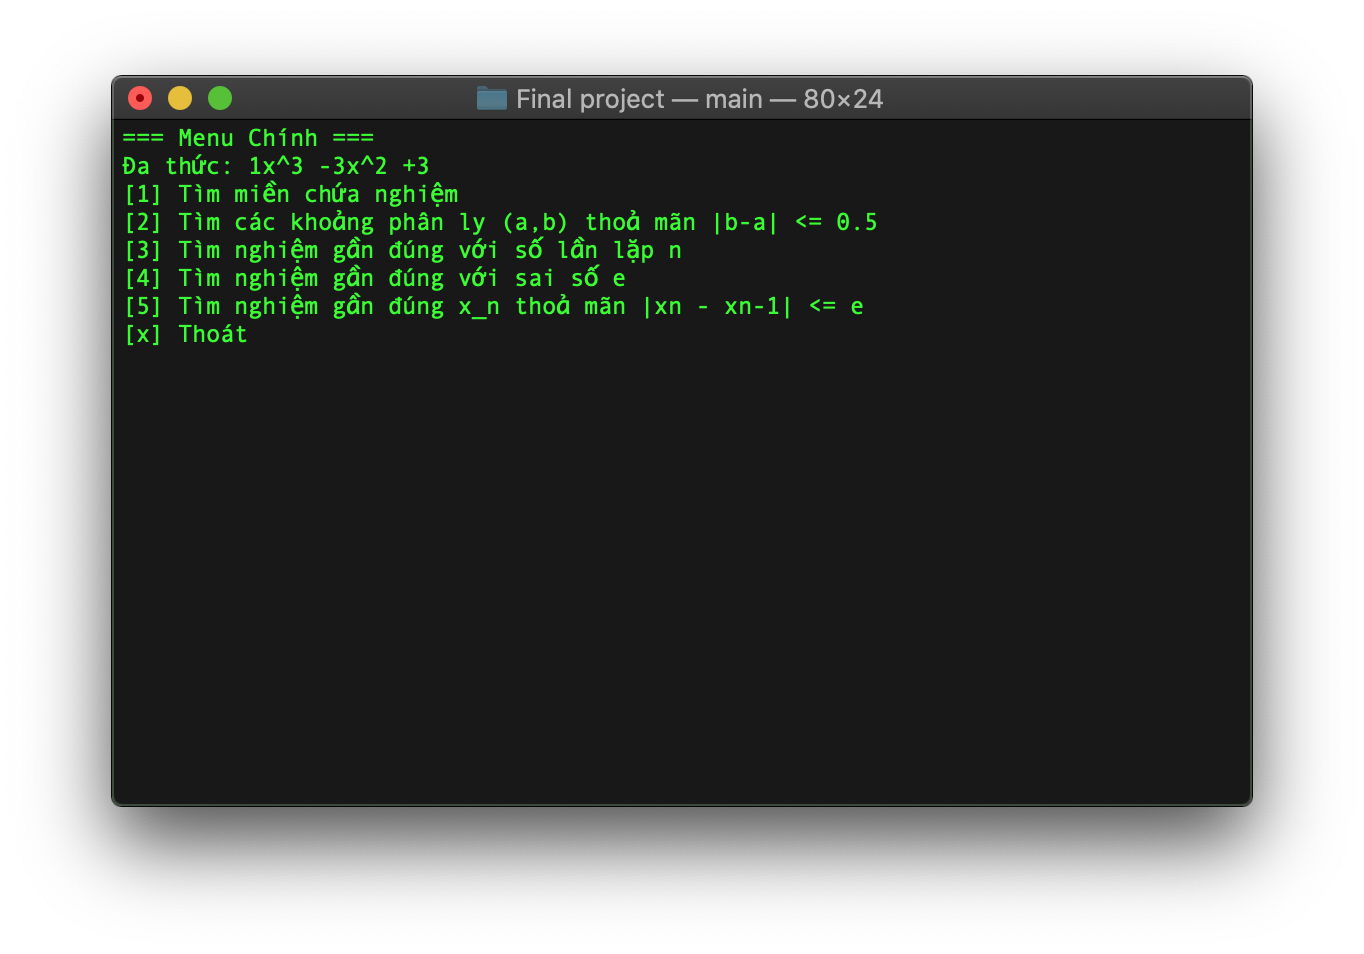
\includegraphics{Report 217e2873af07496eaa16f4f8701bd590/Screen_Shot_2021-06-14_at_02.17.56.png}
\caption{Report\%20217e2873af07496eaa16f4f8701bd590/Screen\_Shot\_2021-06-14\_at\_02.17.56.png}
\end{figure}

\begin{figure}[htbp]
\centering
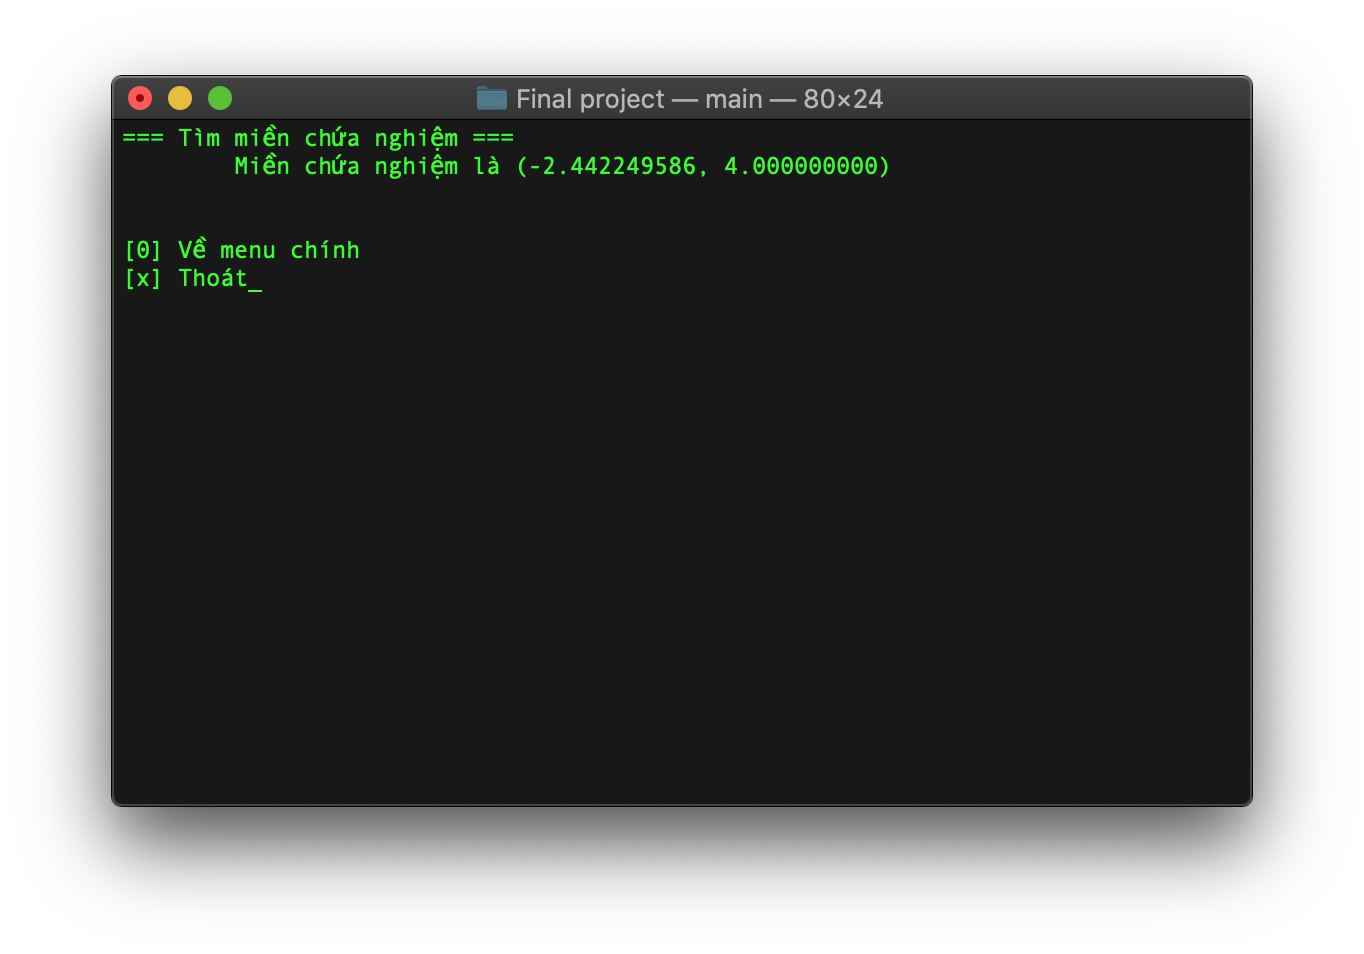
\includegraphics{Report 217e2873af07496eaa16f4f8701bd590/Screen_Shot_2021-06-14_at_02.18.42.png}
\caption{Report\%20217e2873af07496eaa16f4f8701bd590/Screen\_Shot\_2021-06-14\_at\_02.18.42.png}
\end{figure}

\begin{figure}[htbp]
\centering
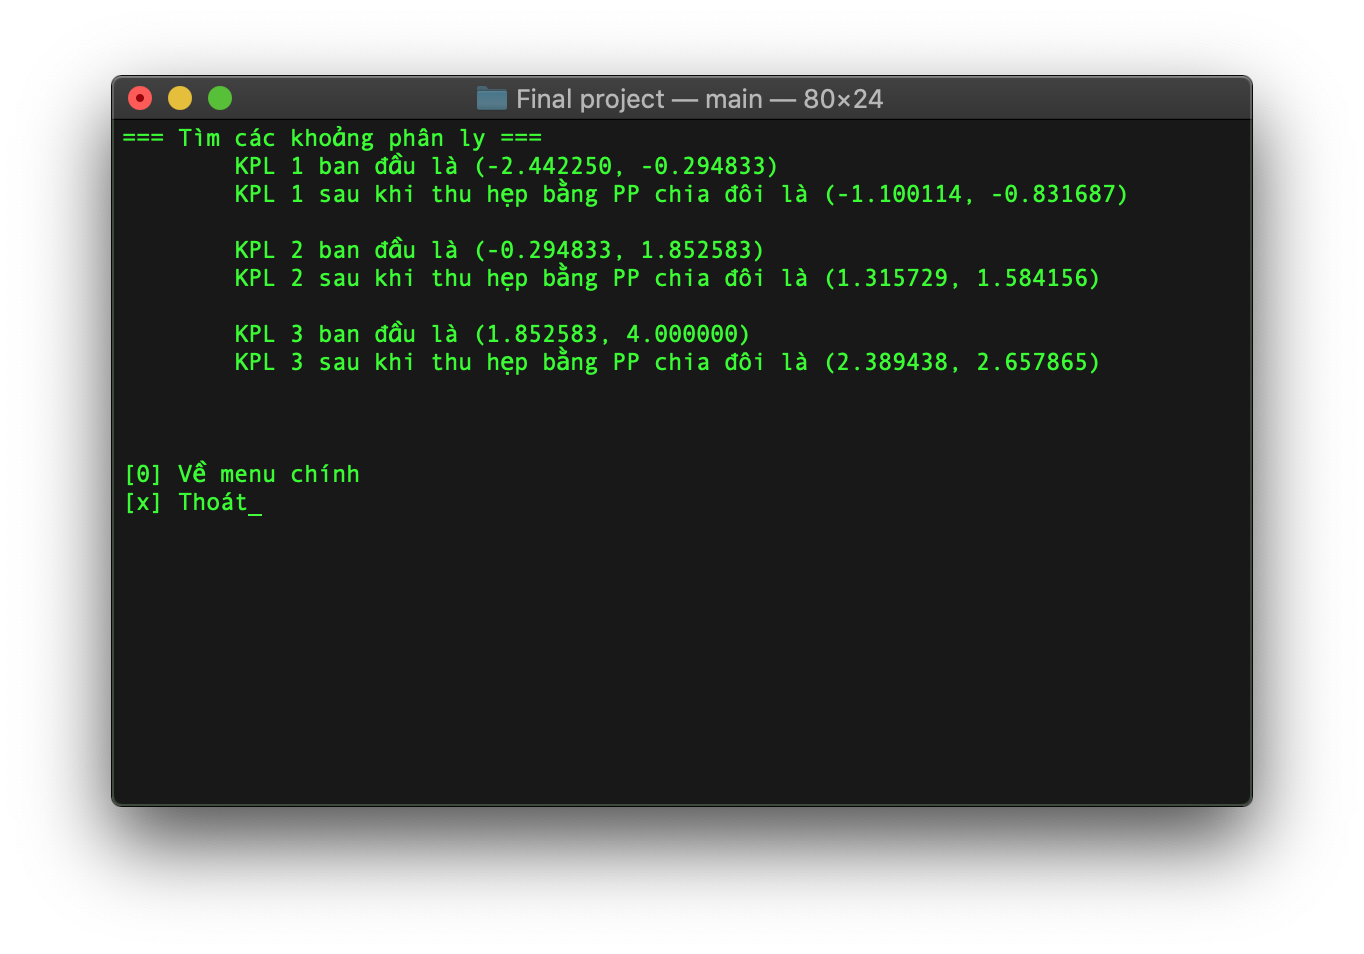
\includegraphics{Report 217e2873af07496eaa16f4f8701bd590/Screen_Shot_2021-06-14_at_02.19.08.png}
\caption{Report\%20217e2873af07496eaa16f4f8701bd590/Screen\_Shot\_2021-06-14\_at\_02.19.08.png}
\end{figure}

\begin{figure}[htbp]
\centering
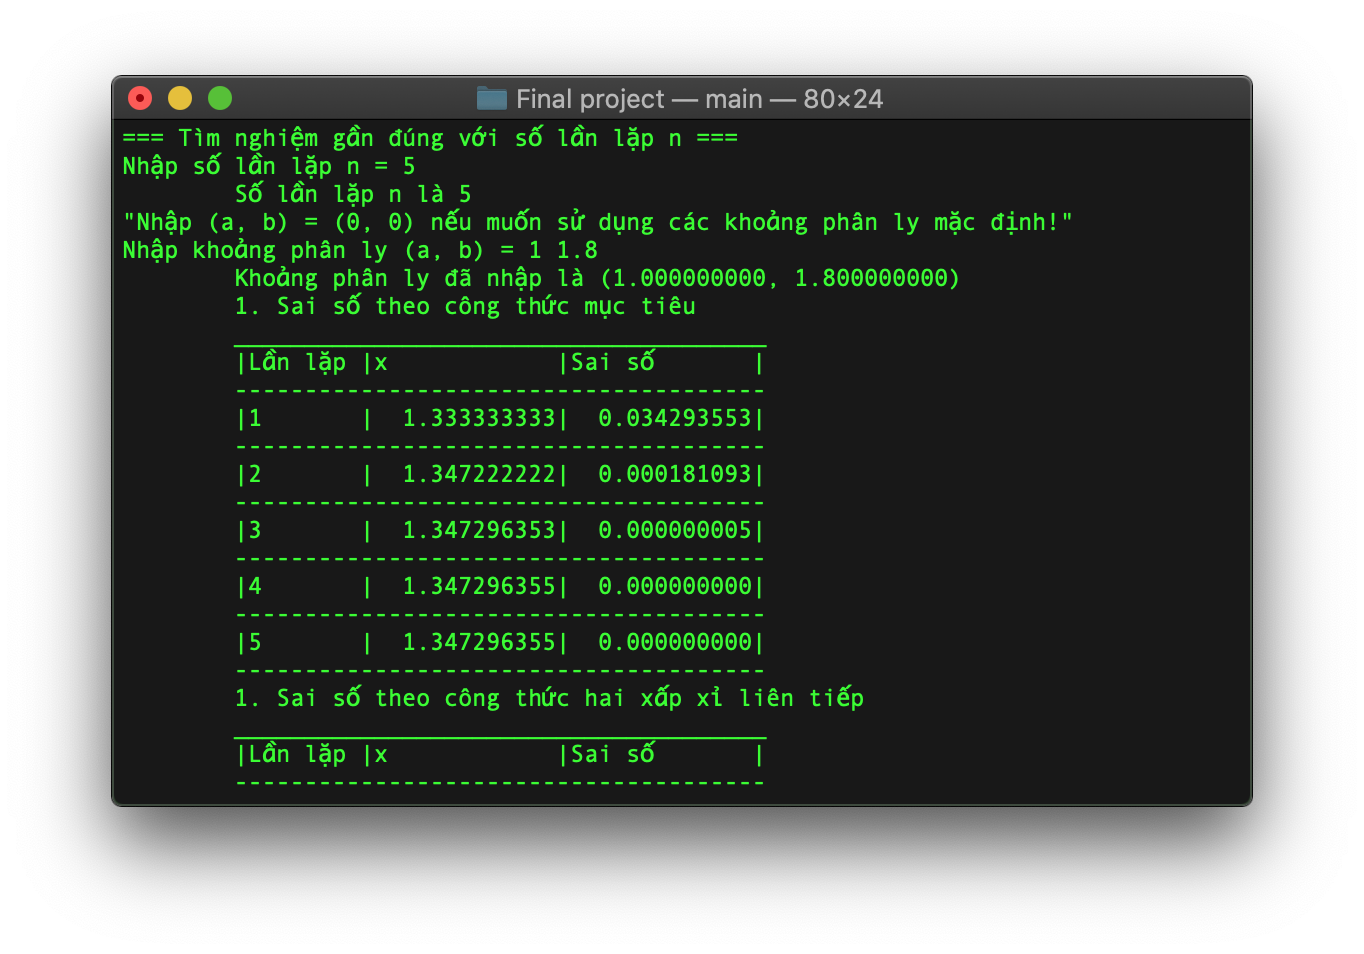
\includegraphics{Report 217e2873af07496eaa16f4f8701bd590/Screen_Shot_2021-06-14_at_02.22.33.png}
\caption{Report\%20217e2873af07496eaa16f4f8701bd590/Screen\_Shot\_2021-06-14\_at\_02.22.33.png}
\end{figure}

\begin{figure}[htbp]
\centering
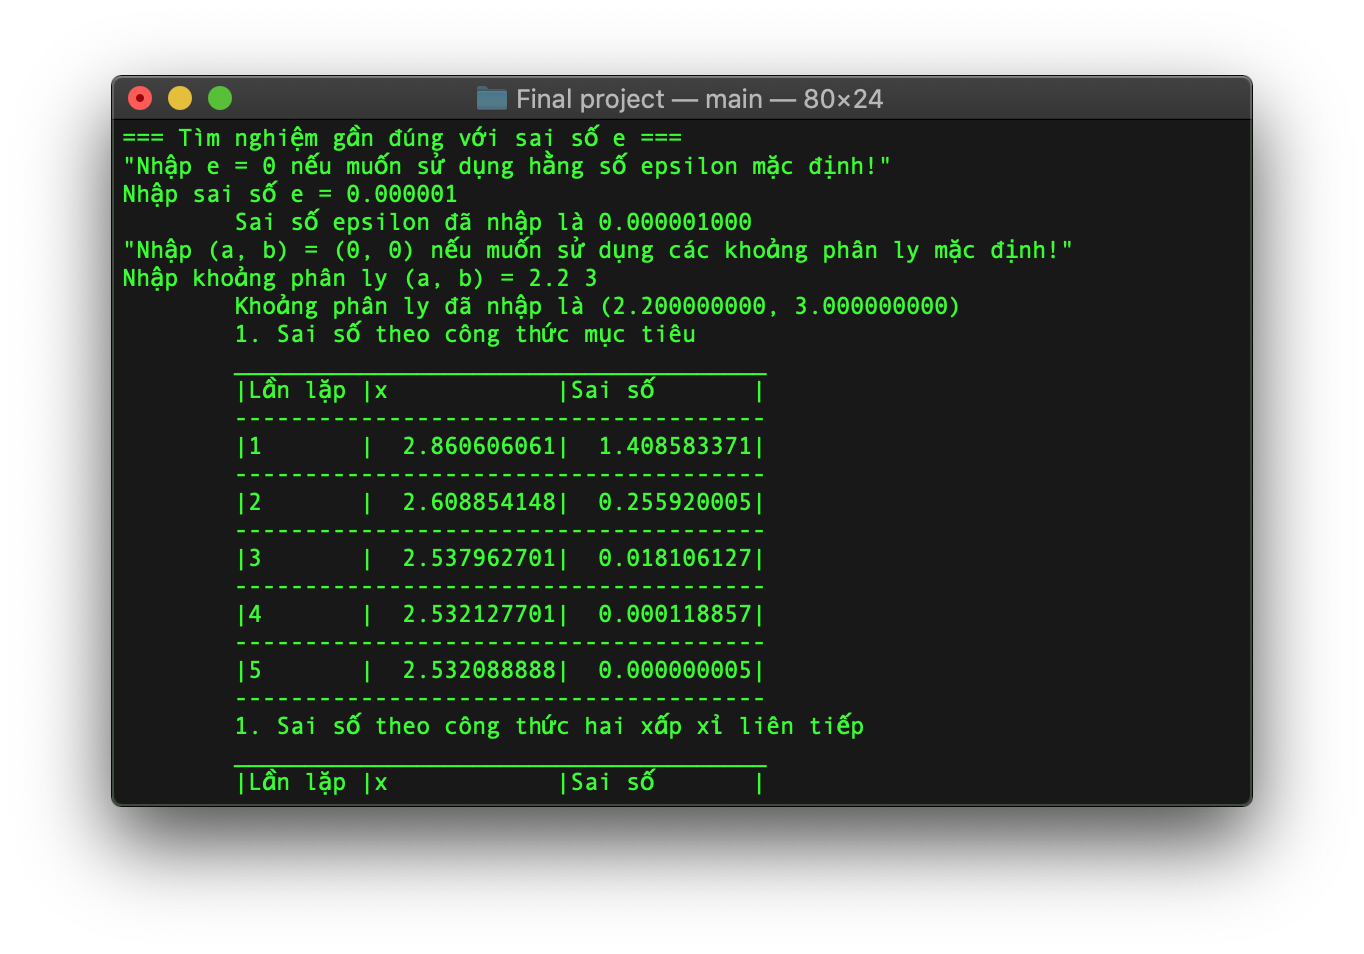
\includegraphics{Report 217e2873af07496eaa16f4f8701bd590/Screen_Shot_2021-06-14_at_02.23.21.png}
\caption{Report\%20217e2873af07496eaa16f4f8701bd590/Screen\_Shot\_2021-06-14\_at\_02.23.21.png}
\end{figure}

\begin{figure}[htbp]
\centering
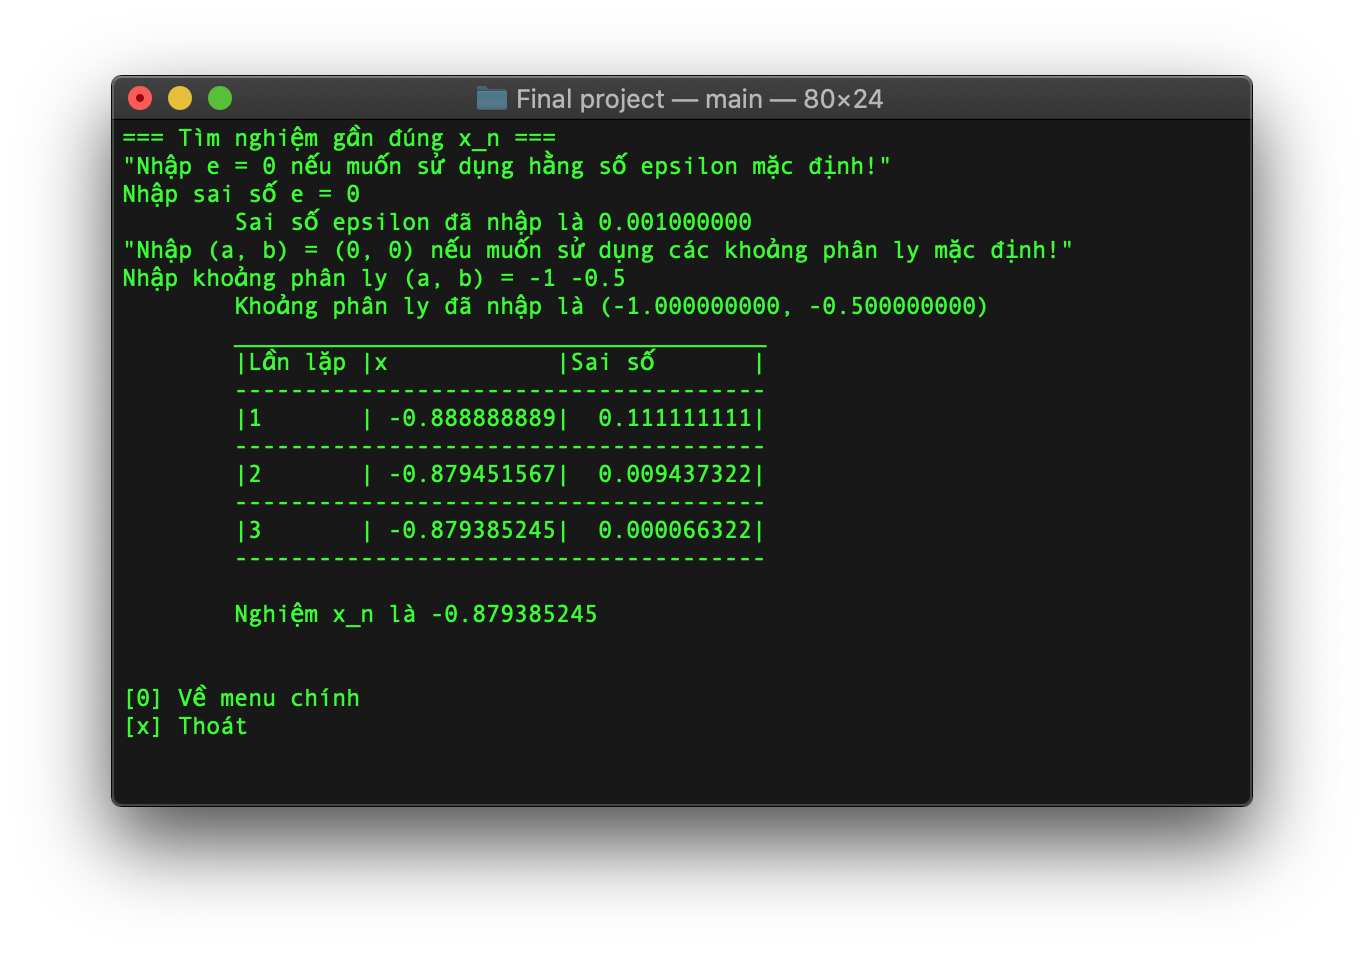
\includegraphics{Report 217e2873af07496eaa16f4f8701bd590/Screen_Shot_2021-06-14_at_02.24.00.png}
\caption{Report\%20217e2873af07496eaa16f4f8701bd590/Screen\_Shot\_2021-06-14\_at\_02.24.00.png}
\end{figure}

\subsection{File quá trình và kết quả
(output.txt)}\label{file-quuxe1-truxecnh-vuxe0-kux1ebft-quux1ea3-output.txt}

\begin{Shaded}
\begin{Highlighting}[]
\NormalTok{Mon Jun }\DecValTok{14} \DecValTok{02}\NormalTok{:}\DecValTok{21}\NormalTok{:}\DecValTok{53} \DecValTok{2021}
    \NormalTok{Khởi tạo chương trình thành công}
\NormalTok{Mon Jun }\DecValTok{14} \DecValTok{02}\NormalTok{:}\DecValTok{21}\NormalTok{:}\DecValTok{59} \DecValTok{2021}
    \NormalTok{Tìm miền chứa nghiệm}
    \NormalTok{Miền chứa nghiệm là (-}\FloatTok{2.442249586}\NormalTok{, }\FloatTok{4.000000000}\NormalTok{)}
\NormalTok{Mon Jun }\DecValTok{14} \DecValTok{02}\NormalTok{:}\DecValTok{22}\NormalTok{:}\DecValTok{05} \DecValTok{2021}
    \NormalTok{Tìm các khoảng phân ly}
    \NormalTok{KPL }\DecValTok{1} \NormalTok{ban đầu là (-}\FloatTok{2.442250}\NormalTok{, -}\FloatTok{0.294833}\NormalTok{)}
    \NormalTok{KPL }\DecValTok{1} \NormalTok{sau khi thu hẹp bằng PP chia đôi là (-}\FloatTok{1.100114}\NormalTok{, -}\FloatTok{0.831687}\NormalTok{)}

    \NormalTok{KPL }\DecValTok{2} \NormalTok{ban đầu là (-}\FloatTok{0.294833}\NormalTok{, }\FloatTok{1.852583}\NormalTok{)}
    \NormalTok{KPL }\DecValTok{2} \NormalTok{sau khi thu hẹp bằng PP chia đôi là (}\FloatTok{1.315729}\NormalTok{, }\FloatTok{1.584156}\NormalTok{)}

    \NormalTok{KPL }\DecValTok{3} \NormalTok{ban đầu là (}\FloatTok{1.852583}\NormalTok{, }\FloatTok{4.000000}\NormalTok{)}
    \NormalTok{KPL }\DecValTok{3} \NormalTok{sau khi thu hẹp bằng PP chia đôi là (}\FloatTok{2.389438}\NormalTok{, }\FloatTok{2.657865}\NormalTok{)}

\NormalTok{Mon Jun }\DecValTok{14} \DecValTok{02}\NormalTok{:}\DecValTok{22}\NormalTok{:}\DecValTok{10} \DecValTok{2021}
    \NormalTok{Tìm nghiệm gần đúng với số lần lặp n}
    \NormalTok{Số lần lặp n là }\DecValTok{5}
    \NormalTok{Khoảng phân ly đã nhập là (}\FloatTok{1.000000000}\NormalTok{, }\FloatTok{1.800000000}\NormalTok{)}
    \DecValTok{1}\NormalTok{. Sai số theo công thức mục tiêu}
    \NormalTok{______________________________________}
    \NormalTok{|Lần lặp |x            |Sai số       |}
    \NormalTok{--------------------------------------}
    \NormalTok{|}\DecValTok{1}       \NormalTok{|  }\FloatTok{1.333333333}\NormalTok{|  }\FloatTok{0.034293553}\NormalTok{|}
    \NormalTok{--------------------------------------}
    \NormalTok{|}\DecValTok{2}       \NormalTok{|  }\FloatTok{1.347222222}\NormalTok{|  }\FloatTok{0.000181093}\NormalTok{|}
    \NormalTok{--------------------------------------}
    \NormalTok{|}\DecValTok{3}       \NormalTok{|  }\FloatTok{1.347296353}\NormalTok{|  }\FloatTok{0.000000005}\NormalTok{|}
    \NormalTok{--------------------------------------}
    \NormalTok{|}\DecValTok{4}       \NormalTok{|  }\FloatTok{1.347296355}\NormalTok{|  }\FloatTok{0.000000000}\NormalTok{|}
    \NormalTok{--------------------------------------}
    \NormalTok{|}\DecValTok{5}       \NormalTok{|  }\FloatTok{1.347296355}\NormalTok{|  }\FloatTok{0.000000000}\NormalTok{|}
    \NormalTok{--------------------------------------}
    \DecValTok{1}\NormalTok{. Sai số theo công thức hai xấp xỉ liên tiếp}
    \NormalTok{______________________________________}
    \NormalTok{|Lần lặp |x            |Sai số       |}
    \NormalTok{--------------------------------------}
    \NormalTok{|}\DecValTok{1}       \NormalTok{|  }\FloatTok{1.333333333}\NormalTok{|  }\FloatTok{0.592592593}\NormalTok{|}
    \NormalTok{--------------------------------------}
    \NormalTok{|}\DecValTok{2}       \NormalTok{|  }\FloatTok{1.347222222}\NormalTok{|  }\FloatTok{0.024691358}\NormalTok{|}
    \NormalTok{--------------------------------------}
    \NormalTok{|}\DecValTok{3}       \NormalTok{|  }\FloatTok{1.347296353}\NormalTok{|  }\FloatTok{0.000131788}\NormalTok{|}
    \NormalTok{--------------------------------------}
    \NormalTok{|}\DecValTok{4}       \NormalTok{|  }\FloatTok{1.347296355}\NormalTok{|  }\FloatTok{0.000000004}\NormalTok{|}
    \NormalTok{--------------------------------------}
    \NormalTok{|}\DecValTok{5}       \NormalTok{|  }\FloatTok{1.347296355}\NormalTok{|  }\FloatTok{0.000000000}\NormalTok{|}
    \NormalTok{--------------------------------------}

    \NormalTok{Nghiệm x là }\FloatTok{1.347296355}
\NormalTok{Mon Jun }\DecValTok{14} \DecValTok{02}\NormalTok{:}\DecValTok{22}\NormalTok{:}\DecValTok{43} \DecValTok{2021}
    \NormalTok{Tìm nghiệm gần đúng với sai số e}
    \NormalTok{Sai số epsilon đã nhập là }\FloatTok{0.000001000}
    \NormalTok{Khoảng phân ly đã nhập là (}\FloatTok{2.200000000}\NormalTok{, }\FloatTok{3.000000000}\NormalTok{)}
    \DecValTok{1}\NormalTok{. Sai số theo công thức mục tiêu}
    \NormalTok{______________________________________}
    \NormalTok{|Lần lặp |x            |Sai số       |}
    \NormalTok{--------------------------------------}
    \NormalTok{|}\DecValTok{1}       \NormalTok{|  }\FloatTok{2.860606061}\NormalTok{|  }\FloatTok{1.408583371}\NormalTok{|}
    \NormalTok{--------------------------------------}
    \NormalTok{|}\DecValTok{2}       \NormalTok{|  }\FloatTok{2.608854148}\NormalTok{|  }\FloatTok{0.255920005}\NormalTok{|}
    \NormalTok{--------------------------------------}
    \NormalTok{|}\DecValTok{3}       \NormalTok{|  }\FloatTok{2.537962701}\NormalTok{|  }\FloatTok{0.018106127}\NormalTok{|}
    \NormalTok{--------------------------------------}
    \NormalTok{|}\DecValTok{4}       \NormalTok{|  }\FloatTok{2.532127701}\NormalTok{|  }\FloatTok{0.000118857}\NormalTok{|}
    \NormalTok{--------------------------------------}
    \NormalTok{|}\DecValTok{5}       \NormalTok{|  }\FloatTok{2.532088888}\NormalTok{|  }\FloatTok{0.000000005}\NormalTok{|}
    \NormalTok{--------------------------------------}
    \DecValTok{1}\NormalTok{. Sai số theo công thức hai xấp xỉ liên tiếp}
    \NormalTok{______________________________________}
    \NormalTok{|Lần lặp |x            |Sai số       |}
    \NormalTok{--------------------------------------}
    \NormalTok{|}\DecValTok{1}       \NormalTok{|  }\FloatTok{2.860606061}\NormalTok{|  }\FloatTok{3.843526171}\NormalTok{|}
    \NormalTok{--------------------------------------}
    \NormalTok{|}\DecValTok{2}       \NormalTok{|  }\FloatTok{2.608854148}\NormalTok{|  }\FloatTok{1.464738402}\NormalTok{|}
    \NormalTok{--------------------------------------}
    \NormalTok{|}\DecValTok{3}       \NormalTok{|  }\FloatTok{2.537962701}\NormalTok{|  }\FloatTok{0.412459330}\NormalTok{|}
    \NormalTok{--------------------------------------}
    \NormalTok{|}\DecValTok{4}       \NormalTok{|  }\FloatTok{2.532127701}\NormalTok{|  }\FloatTok{0.033949089}\NormalTok{|}
    \NormalTok{--------------------------------------}
    \NormalTok{|}\DecValTok{5}       \NormalTok{|  }\FloatTok{2.532088888}\NormalTok{|  }\FloatTok{0.000225821}\NormalTok{|}
    \NormalTok{--------------------------------------}
    \NormalTok{|}\DecValTok{6}       \NormalTok{|  }\FloatTok{2.532088886}\NormalTok{|  }\FloatTok{0.000000010}\NormalTok{|}
    \NormalTok{--------------------------------------}

    \NormalTok{Nghiệm x là }\FloatTok{2.532088886}
\NormalTok{Mon Jun }\DecValTok{14} \DecValTok{02}\NormalTok{:}\DecValTok{23}\NormalTok{:}\DecValTok{29} \DecValTok{2021}
    \NormalTok{Tìm nghiệm gần đúng x_n}
    \NormalTok{Sai số epsilon đã nhập là }\FloatTok{0.001000000}
    \NormalTok{Khoảng phân ly đã nhập là (-}\FloatTok{1.000000000}\NormalTok{, -}\FloatTok{0.500000000}\NormalTok{)}
    \NormalTok{______________________________________}
    \NormalTok{|Lần lặp |x            |Sai số       |}
    \NormalTok{--------------------------------------}
    \NormalTok{|}\DecValTok{1}       \NormalTok{| -}\FloatTok{0.888888889}\NormalTok{|  }\FloatTok{0.111111111}\NormalTok{|}
    \NormalTok{--------------------------------------}
    \NormalTok{|}\DecValTok{2}       \NormalTok{| -}\FloatTok{0.879451567}\NormalTok{|  }\FloatTok{0.009437322}\NormalTok{|}
    \NormalTok{--------------------------------------}
    \NormalTok{|}\DecValTok{3}       \NormalTok{| -}\FloatTok{0.879385245}\NormalTok{|  }\FloatTok{0.000066322}\NormalTok{|}
    \NormalTok{--------------------------------------}

    \NormalTok{Nghiệm x_n là -}\FloatTok{0.879385245}
\NormalTok{Mon Jun }\DecValTok{14} \DecValTok{02}\NormalTok{:}\DecValTok{24}\NormalTok{:}\DecValTok{06} \DecValTok{2021}
    \NormalTok{Kết thúc chương trình}
\end{Highlighting}
\end{Shaded}

